% ═══════════════════════════════════════════════════════════════════════════════
%  OTC-X  ·  Liquidity Intelligence Radar
%  ─────────────────────────────────────────────────────────────────────────────
%  Market-Intelligence Dossier — Operational Evidence for Swiss OTC Equities
%  Requirements Engineering Katalog nach IREB (CPRE-FL)  ·  Quantitative Methodik
%  ─────────────────────────────────────────────────────────────────────────────
%  Autor:           Mihael Atanasov
%  Version:         3.1  ·  August 2026  (Market-Intelligence Edition · Projektkontext richtiggestellt)
%  Klassifikation:  Proprietär & Vertraulich
%  Build engine:    LuaLaTeX  +  fontspec  +  unicode-math
% ═══════════════════════════════════════════════════════════════════════════════

\documentclass[11pt, a4paper, oneside, openany]{report}

% ── LuaLaTeX modern font stack via fontspec ─────────────────────────────────
\usepackage{fontspec}
\usepackage[ngerman]{babel}

% Body — IBM Plex Serif (institutional readability + true German diacritics + ẞ)
\setmainfont{IBM Plex Serif}[
  Numbers={Tabular,Lining},
  Ligatures=TeX,
]

% Headings — Inter (Display optical size where available)
\setsansfont{Inter}[
  Numbers={Tabular,Lining},
  Ligatures=TeX,
]

% Mono-data — IBM Plex Mono, programming ligatures DISABLED (ISINs, prices, IDs)
\setmonofont{IBM Plex Mono}[
  Numbers={Tabular,Lining},
  RawFeature={-calt;-liga},
  Scale=0.92,
]

% Mono-data macro family (ISINs / prices / IDs — explicit when not in \texttt)
\newfontfamily\datafont{IBM Plex Mono}[
  Numbers={Tabular,Lining},
  RawFeature={-calt;-liga},
  Scale=0.92,
]

% Mono-code — JetBrains Mono with programming ligatures (code listings only)
\newfontfamily\codefont{JetBrains Mono}[
  Scale=0.88,
  Ligatures=TeX,
]

% Math — traditional amsmath/amssymb stack (Latin Modern Math) for stability;
% body & display fonts come from fontspec above. This hybrid trades the visual
% lift of STIX Two for full compatibility with existing \mathbb{1}, \blacksquare,
% indicator functions and ams* macros referenced in the methodology chapter.

% Microtype & spacing
\usepackage{microtype}
\usepackage{setspace}
\onehalfspacing
\usepackage{parskip}
\usepackage{lettrine}
\usepackage{epigraph}
\setlength{\epigraphwidth}{0.66\textwidth}
\setlength{\epigraphrule}{0.4pt}
\renewcommand{\epigraphflush}{flushleft}
\renewcommand{\sourceflush}{flushleft}

% ── Page Geometry — symmetric, full body width (final submission layout) ──
\usepackage[
  paperwidth=210mm,
  paperheight=297mm,
  top=26mm, bottom=28mm,
  inner=25mm, outer=25mm,
  headheight=22pt,
  headsep=8mm,
  footskip=12mm,
]{geometry}

% ── v3.0 Colour System — three functional palettes + neutral ramp ──────────
\usepackage[dvipsnames,svgnames,x11names]{xcolor}

% Identity palette — restraint, ≤2% page ink coverage target
\definecolor{SwissRed}{HTML}{B22222}
\definecolor{DeepNavy}{HTML}{1A1A2E}
\definecolor{LightSilver}{HTML}{F5F6F8}

% Data palette — charts, KPI tiles, hyperlinks
\definecolor{MetricBlue}{HTML}{2B6CB0}
\definecolor{AccentGold}{HTML}{A0B800}
\definecolor{LinkBlue}{HTML}{2E86AB}

% Trust palette — severity 6-step (Clean → Extreme), refined v3.0
\definecolor{SevClean}{HTML}{2F855A}
\definecolor{SevWatch}{HTML}{A0B800}
\definecolor{SevAlert}{HTML}{D69E2E}
\definecolor{SevCritical}{HTML}{DD6B20}
\definecolor{SevSevere}{HTML}{C53030}
\definecolor{SevExtreme}{HTML}{742A2A}

% Neutral grayscale ramp — data ink, marginalia, gridlines
\definecolor{N100}{HTML}{F7FAFC}
\definecolor{N200}{HTML}{EDF2F7}
\definecolor{N300}{HTML}{E2E8F0}
\definecolor{N400}{HTML}{CBD5E0}
\definecolor{N500}{HTML}{A0AEC0}
\definecolor{N600}{HTML}{718096}
\definecolor{N700}{HTML}{4A5568}
\definecolor{N800}{HTML}{2D3748}
\definecolor{N900}{HTML}{1A202C}

% Backward-compatibility aliases (v2.2 body refers to these names)
\colorlet{WarnAmber}{SevAlert}
\colorlet{CriticalOrange}{SevCritical}
\colorlet{SevereRed}{SevSevere}
\colorlet{CleanGreen}{SevClean}
\colorlet{SlateGrey}{N700}
\colorlet{CodeBg}{N100}

% ── Headers & Footers — v3.0 with build identity ───────────────────────────
\usepackage{fancyhdr}
\pagestyle{fancy}
\fancyhf{}
\renewcommand{\headrulewidth}{0.4pt}
\renewcommand{\footrulewidth}{0pt}
\renewcommand{\headrule}{\hbox to\headwidth{%
  \color{SwissRed}\leaders\hrule height \headrulewidth\hfill}}
\fancyhead[L]{\small\sffamily\textcolor{SwissRed}{\textbf{OTC\,|\,X}}}
\fancyhead[R]{\small\sffamily\textcolor{N700}{\nouppercase{\leftmark}}}
\fancyfoot[C]{\small\sffamily\textcolor{DeepNavy}{\thepage}}
\fancyfoot[L]{\tiny\datafont\textcolor{N600}{build~37b425e}}
\fancyfoot[R]{\tiny\sffamily\textcolor{N700}{v3.1 · August 2026}}

% ── Mathematics — classical ams stack (Latin Modern Math) ────────────────
\usepackage{amsmath, amssymb, amsthm, mathtools}
\usepackage{bm}

% ── Graphics, Tables & TikZ — v3.0 with pgfgantt + pgf-pie + calendar ──────
\usepackage{graphicx}
\usepackage{booktabs}
\usepackage{tabularx}
\usepackage{longtable}
\usepackage{multirow}
\usepackage{colortbl}
\usepackage{array}
\usepackage{float}
\usepackage{nicematrix}
\usepackage{caption}
\captionsetup{
  font={small,sf},
  labelfont={bf,color=SwissRed},
  format=hang,
  margin=1cm,
}

\usepackage{tikz}
\usetikzlibrary{shapes.geometric, arrows.meta, positioning, calc, fit, backgrounds,
                decorations.pathreplacing, patterns, calendar}
\usepackage{pgfplots}
\pgfplotsset{compat=1.18}
\usepackage{pgfgantt}
\usepackage{pgf-pie}

% ── Margin column system — marginnote (governed placement) ─────────────────
\usepackage{marginnote}
\renewcommand*{\marginfont}{\footnotesize\sffamily\color{N700}}

% Kennzahl margin macro — verifiable mini-stat, mono number + uppercase label
\newcommand{\kpi}[2]{\marginnote{%
  {\sffamily\scriptsize\bfseries\color{N700}\MakeUppercase{#1}}\par
  {\datafont\fontsize{11}{13}\selectfont\color{N900}#2}%
}}

% Requirement margin anchor — echoes FA/NFA/C ID in margin for audit scannability
\newcommand{\reqanchor}[1]{\marginnote{%
  {\datafont\footnotesize\bfseries\color{SwissRed}#1}%
}}

% ── Boxes & Environments ────────────────────────────────────────────────────
\usepackage[most]{tcolorbox}
\tcbset{
  sharp corners,
  boxrule=0pt,
  left=8pt, right=8pt, top=6pt, bottom=6pt,
  fonttitle=\sffamily\bfseries,
}

\newtcolorbox{reqbox}[1][]{
  colback=LightSilver,
  colframe=SwissRed,
  borderline west={3pt}{0pt}{SwissRed},
  title={#1},
  coltitle=white,
  colbacktitle=SwissRed,
  fonttitle=\sffamily\bfseries\small,
  arc=1.5mm,
  boxrule=0.6pt,
}

\newtcolorbox{infobox}[1][]{
  colback=MetricBlue!4,
  colframe=MetricBlue,
  borderline west={3pt}{0pt}{MetricBlue},
  title={#1},
  coltitle=white,
  colbacktitle=MetricBlue,
  fonttitle=\sffamily\bfseries\small,
  arc=1.5mm,
  boxrule=0.6pt,
}

\newtcolorbox{mathbox}[1][]{
  colback=LightSilver,
  colframe=DeepNavy,
  borderline west={3pt}{0pt}{DeepNavy},
  title={#1},
  coltitle=white,
  colbacktitle=DeepNavy,
  fonttitle=\sffamily\bfseries\small,
  arc=1.5mm,
  boxrule=0.6pt,
}

\newtcolorbox{warnbox}[1][]{
  colback=SevSevere!4,
  colframe=SevSevere,
  borderline west={3pt}{0pt}{SevSevere},
  title={#1},
  coltitle=white,
  colbacktitle=SevSevere,
  fonttitle=\sffamily\bfseries\small,
  arc=1.5mm,
  boxrule=0.6pt,
}

\newtcolorbox{insightbox}[1][]{
  colback=AccentGold!8,
  colframe=AccentGold!70!black,
  boxrule=0.5pt,
  arc=2mm,
  left=6pt, right=6pt, top=4pt, bottom=4pt,
  fontupper=\itshape,
  #1
}

\newtcolorbox{constraintbox}[1][]{
  colback=SevAlert!8,
  colframe=SevAlert!80!black,
  borderline west={3pt}{0pt}{SevAlert!80!black},
  title={#1},
  fonttitle=\sffamily\bfseries\small,
  boxrule=0.5pt,
  arc=1.5mm,
  left=6pt, right=6pt, top=4pt, bottom=4pt,
}

% ── Listings — JetBrains Mono for code, ligatures preserved ────────────────
\usepackage{listings}
\lstdefinestyle{otcx}{
  basicstyle=\codefont\small,
  backgroundcolor=\color{N100},
  frame=single,
  rulecolor=\color{N300},
  keywordstyle=\color{MetricBlue}\bfseries,
  commentstyle=\color{N600}\itshape,
  stringstyle=\color{SwissRed},
  breaklines=true,
  numbers=left,
  numberstyle=\tiny\codefont\color{N500},
  tabsize=4,
  showstringspaces=false,
  xleftmargin=1.5em,
  framexleftmargin=1em,
  aboveskip=1em,
  belowskip=0.8em,
}
\lstset{style=otcx}

% ── Hyperlinks ──────────────────────────────────────────────────────────────
\usepackage[
  colorlinks=true,
  linkcolor=SwissRed,
  urlcolor=LinkBlue,
  citecolor=DeepNavy,
  bookmarks=true,
  bookmarksopen=true,
  pdfauthor={Mihael Atanasov},
  pdftitle={OTC-X Market-Intelligence Dossier · v3.1},
  pdfsubject={Requirements Engineering nach IREB · Operational Evidence · Schweizer OTC-Markt (OTC-X)},
]{hyperref}
\usepackage{bookmark}

% ── Lists ───────────────────────────────────────────────────────────────────
\usepackage{enumitem}
\setlist[itemize]{leftmargin=1.5em, itemsep=2pt}
\setlist[enumerate]{leftmargin=1.8em, itemsep=2pt}

% ── Section Styling ─────────────────────────────────────────────────────────
\usepackage{titlesec}

\titleformat{\chapter}[display]
  {\normalfont\huge\bfseries\sffamily\color{DeepNavy}}
  {\textcolor{SwissRed}{\rule{4pt}{1.5cm}}\quad\LARGE\textcolor{SwissRed}{Kapitel \thechapter}}
  {0.5em}
  {}
  [\vspace{-0.5em}{\color{SwissRed}\rule{\textwidth}{1pt}}]

\titleformat{\section}
  {\normalfont\Large\bfseries\sffamily\color{DeepNavy}}
  {\textcolor{SwissRed}{\thesection}}{0.8em}{}

\titleformat{\subsection}
  {\normalfont\large\bfseries\sffamily\color{DeepNavy}}
  {\textcolor{SwissRed}{\thesubsection}}{0.7em}{}

\titleformat{\subsubsection}
  {\normalfont\normalsize\bfseries\sffamily\color{SlateGrey}}
  {\textcolor{SwissRed}{\thesubsubsection}}{0.6em}{}

% ── Glossary ────────────────────────────────────────────────────────────────
\usepackage[acronym,toc]{glossaries}
\makeglossaries

\newacronym{ireb}{IREB}{International Requirements Engineering Board}
\newacronym{otcx}{OTC-X}{Over-the-Counter Exchange (Berner Börse)}
\newacronym{bekb}{BEKB}{Berner Kantonalbank AG}
\newacronym{isin}{ISIN}{International Securities Identification Number}
\newacronym{etl}{ETL}{Extract, Transform, Load}
\newacronym{chf}{CHF}{Schweizer Franken}
\newacronym{api}{API}{Application Programming Interface}
\newacronym{ci}{CI}{Continuous Integration}
\newacronym{cd}{CD}{Continuous Deployment}

% ── Shorthand Commands ──────────────────────────────────────────────────────
\newcommand{\term}[1]{\textcolor{SwissRed}{\sffamily\textbf{#1}}}
\newcommand{\code}[1]{{\codefont\small\textcolor{DeepNavy}{#1}}}
\newcommand{\metr}[1]{{\datafont\footnotesize\textcolor{MetricBlue}{#1}}}
\newcommand{\datavalue}[1]{{\datafont\textcolor{N900}{#1}}}
\newcommand{\isin}[1]{{\datafont\textcolor{N900}{#1}}}

% ═════════════════════════════════════════════════════════════════════════════
%  DOCUMENT START
% ═════════════════════════════════════════════════════════════════════════════
\begin{document}

% ── TITLE PAGE — v3.0 Market-Intelligence Dossier Cover ────────────────────
% Tier 2 SIX/Bloomberg dossier: 7-zone vertical structure, kennzahl strip with
% REPO-VERIFIED values only, mono accents, single-accent Swiss Red discipline.
\begin{titlepage}
\newgeometry{top=20mm, bottom=20mm, left=22mm, right=22mm}
\pagestyle{empty}

% Zone A — Classification bar (6mm)
\noindent\textcolor{N700}{\sffamily\fontsize{7.5}{9}\selectfont\bfseries
PROPRIETÄR \& VERTRAULICH \quad\textcolor{SwissRed}{\rule[0.5ex]{8pt}{1pt}}\quad
MARKET-INTELLIGENCE DOSSIER \quad\textcolor{SwissRed}{\rule[0.5ex]{8pt}{1pt}}\quad
v3.1\,/\,AUGUST 2026}
\vspace{3mm}
\noindent\textcolor{N300}{\rule{\textwidth}{0.4pt}}

\vspace{18mm}

% Zone B — Identity block (52mm): OTC | X mark + dossier label, flush left
\noindent{\sffamily\fontsize{72}{80}\selectfont\bfseries\color{DeepNavy}OTC\,\textcolor{SwissRed}{|}\,X}\\[2pt]
\noindent{\datafont\fontsize{8.5}{12}\selectfont\color{N700}\MakeUppercase{Liquidity Intelligence Radar \,/\, Swiss OTC Equities}}

\vspace{28mm}

% Zone C — Title block (70mm)
\noindent{\sffamily\fontsize{38}{44}\selectfont\bfseries\color{DeepNavy}Anforderungskatalog}\\[4mm]
\noindent{\sffamily\fontsize{13}{16}\selectfont\itshape\color{N700}IREB-konforme Spezifikation, quantitative Methodik\\
und operationelle Evidenz\,---\,ein unabhängiges Projekt zum \mbox{OTC-X}-Markt.}

\vspace{14mm}

% Zone D — Kennzahl Strip (38mm): four cells of repo-verified facts
\noindent\textcolor{N300}{\rule{\textwidth}{0.4pt}}\\[1mm]
\noindent{\sffamily\fontsize{6.5}{8}\selectfont\color{N600}\MakeUppercase{Operational evidence \,/\, repo-verified \,/\, build~37b425e}}\\[3mm]
\noindent\begin{tabular*}{\textwidth}{@{\extracolsep{\fill}}llll@{}}
{\datafont\fontsize{26}{30}\selectfont\color{DeepNavy}243} &
{\datafont\fontsize{26}{30}\selectfont\color{DeepNavy}22\,+} &
{\datafont\fontsize{26}{30}\selectfont\color{DeepNavy}54} &
{\datafont\fontsize{26}{30}\selectfont\color{DeepNavy}115} \\[1mm]
{\sffamily\fontsize{7}{9}\selectfont\color{N700}\MakeUppercase{Wertpapiere im Universum}} &
{\sffamily\fontsize{7}{9}\selectfont\color{N700}\MakeUppercase{Jahre Handelshistorie}} &
{\sffamily\fontsize{7}{9}\selectfont\color{N700}\MakeUppercase{Zero-Touch Pipeline-Läufe}} &
{\sffamily\fontsize{7}{9}\selectfont\color{N700}\MakeUppercase{CI-gegatete Tests}} \\
\end{tabular*}\\[2mm]
\noindent\textcolor{N300}{\rule{\textwidth}{0.4pt}}

\vfill

% Zone F — Metadata footer
\noindent\textcolor{DeepNavy}{\rule{30mm}{2pt}}\\[3mm]
\noindent\begin{tabular}{@{}p{32mm}@{\hskip 6pt}p{0.7\textwidth}@{}}
{\sffamily\fontsize{7.5}{10}\selectfont\bfseries\color{N700}\MakeUppercase{Autor}} & {\sffamily\small Mihael Atanasov \quad \textcolor{N600}{\datafont\footnotesize\href{mailto:mihaelatanasov22@gmail.com}{mihaelatanasov22@gmail.com}}} \\
{\sffamily\fontsize{7.5}{10}\selectfont\bfseries\color{N700}\MakeUppercase{Projektkontext}} & {\sffamily\small Unabhängiges Eigenprojekt\,---\,kein Auftragsverhältnis \quad \textcolor{N600}{\sffamily\footnotesize Berner Kantonalbank AG als potenzielle Empfängerin bzw.\ Interessentin}} \\
{\sffamily\fontsize{7.5}{10}\selectfont\bfseries\color{N700}\MakeUppercase{Domäne}} & {\sffamily\small Schweizer OTC-Aktien — 243 ausserbörsliche Titel, 224 mit aktiver Handelshistorie} \\
{\sffamily\fontsize{7.5}{10}\selectfont\bfseries\color{N700}\MakeUppercase{Version}} & {\datafont\small v3.1 \quad \textcolor{N600}{\sffamily\footnotesize Market-Intelligence Edition}} \\
{\sffamily\fontsize{7.5}{10}\selectfont\bfseries\color{N700}\MakeUppercase{Datenstand}} & {\datafont\small 2026-05-14 \quad \textcolor{N600}{\sffamily\footnotesize letzte automatisierte Pipeline}} \\
{\sffamily\fontsize{7.5}{10}\selectfont\bfseries\color{N700}\MakeUppercase{Build}} & {\datafont\small commit~37b425e \quad \textcolor{N600}{\sffamily\footnotesize LuaLaTeX · fontspec · IBM Plex + Inter}} \\
{\sffamily\fontsize{7.5}{10}\selectfont\bfseries\color{N700}\MakeUppercase{Klassifikation}} & {\sffamily\small\bfseries\color{SwissRed}Proprietär \& Vertraulich} \\
\end{tabular}

\vspace{8mm}

% Zone G — Verification line
\noindent\textcolor{N300}{\rule{\textwidth}{0.3pt}}\\[1.5mm]
\noindent{\datafont\fontsize{6.5}{8}\selectfont\color{N600}%
github.com/atanasovmi/OTC-X \quad·\quad otc-x-radar.streamlit.app \quad·\quad LuaLaTeX-build \quad·\quad reproducible from source}

\restoregeometry
\end{titlepage}

% ── FRONT MATTER ────────────────────────────────────────────────────────────
\pagenumbering{roman}

% ═════════════════════════════════════════════════════════════════════════════
%  INVESTOREN-BRIEFING — Kompakte Investitionsthese (eine Seite)
% ═════════════════════════════════════════════════════════════════════════════
\chapter*{Investoren-Briefing}
\addcontentsline{toc}{chapter}{Investoren-Briefing}

\vspace{-0.4cm}
\noindent{\small\sffamily\textcolor{SlateGrey}{Kompaktes Lagebild für Entscheidungsträger\;\textbullet\;Stand: Mai 2026}}

\vspace{0.8cm}

% Kennzahlen-Ribbon hier entfernt — bereits auf Cover-Strip dargestellt.

\noindent\textbf{\sffamily\textcolor{SwissRed}{Problemraum.}}\;Der Schweizer ausserbörsliche Aktienhandel\,---\,repräsentiert durch die OTC-X-Plattform der Berner Kantonalbank\,---\,ist die letzte signifikante Liquiditätsquelle des Landes ohne institutionalisierte, systematische Überwachung. Fragmentierte Datenströme, fehlende standardisierte Liquiditätsmetriken und blinde Anomalie-Signale erzwingen ein erfahrungsbasiertes \glqq Bauchgefühl-Trading\grqq{} bei einem Marktsegment, das jede manuelle Beobachtung systematisch unterläuft.

\vspace{0.35cm}

\noindent\textbf{\sffamily\textcolor{SwissRed}{Lösung.}}\;\term{OTC-X Liquidity Intelligence Radar} transformiert diese Opazität in einen täglich aktualisierten Decision-Support-Layer: \textbf{26 quantitative Kennzahlen} pro ISIN und Handelstag (inkl. Amihud-Illiquiditätsratio, Corwin--Schultz-Spread-Proxy, EWMA-geglätteter Volatilitätsregime), \textbf{gewichtetes Anomaly-Scoring} mit sechs Severity-Stufen sowie ein \textbf{4-Tab-Dashboard} mit elf interaktiven Chart-Typen\,---\,vollständig automatisiert, mathematisch begründet, regulatorisch auditierbar.

\vspace{0.35cm}

\noindent\textbf{\sffamily\textcolor{SwissRed}{Validierung \& Status.}}
\begin{itemize}[leftmargin=1.4em, itemsep=2pt, topsep=2pt]
  \item \textbf{Projektstatus:}\;Unabhängig konzipiert und umgesetzt\,---\,ohne Auftrag, Mandat oder Mitwirkung der \gls{bekb}. Die \gls{bekb} ist ausschliesslich als potenzielle Empfängerin bzw.\ Interessentin adressiert.
  \item \textbf{Institutionelle Autorisierung:}\;Explizite Datenverarbeitungs-Erlaubnis durch die \gls{bekb} (Schwarzenburgstrasse 160, 3001 Bern) für die Dauer der Entwicklung.
  \item \textbf{Produktivbetrieb:}\;Tägliche zero-touch Pipeline-Läufe seit 29.\,März 2026; aktuell \textbf{54 konsekutive Erfolge} ohne manuellen Eingriff. Live-Demonstrations-Dashboard öffentlich zugänglich unter \href{https://otc-x-radar.streamlit.app}{otc-x-radar.streamlit.app} (kontrolliertes Read-Only-Layer ohne API- oder Daten-Export).
  \item \textbf{Banking-Grade Lieferkette:}\;Cosign-signierte Multi-Arch-Container-Images (linux/amd64 + linux/arm64) auf GHCR, mit SBOM und SLSA-Provenance-Attestationen\,---\,lückenlose Auditierbarkeit vom Container-Digest bis zum Source-Commit (vgl.~Abschnitt~\ref{sec:supplychain}).
  \item \textbf{Normative Konformität:}\;Vollständige Dokumentation nach IREB CPRE Foundation Level (Syllabus~v3.1.2) mit Traceability Matrix\,---\,siehe das vorliegende Werk.
\end{itemize}

\vspace{0.4cm}

\noindent\textbf{\sffamily\textcolor{SwissRed}{Ausblick.}}\;Die Plattform expandiert entlang dreier strategischer Säulen: \textit{prädiktive Liquiditätsanalytik} (Phase~1, Q3--Q4 2026), \textit{marktübergreifende Anreicherung} mit SIX- und SNB-Referenzdaten (Phase~2, Q1--Q2 2027) und \textit{Echtzeit-Streaming} via WebSocket-Feeds (Phase~3, Q3--Q4 2027). Die übergeordnete Vision\,---\,detailliert in Kapitel~\ref{ch:roadmap}\,---\,ist die Etablierung von OTC-X als institutionelles Decision-Support-System für sämtliche Schweizer ausserbörsliche Märkte.

\vspace{0.55cm}

\begin{insightbox}
Der OTC-X-Markt wird seit über zwei Jahrzehnten durch die Berner Kantonalbank betrieben\,---\,aber erst die hier vorgestellte Plattform macht ihn quantitativ \emph{lesbar}. Was bislang einer kleinen Gruppe erfahrener Händler vorbehalten war, wird nun zu einem datengestützten, reproduzierbaren und auditierbaren Prozess. Das ist nicht eine Verbesserung des bestehenden Workflows\,---\,es ist die erste vollständige Quantifizierung eines bisher opaken Marktes.
\end{insightbox}

\clearpage

% ── MANAGEMENT SUMMARY ─────────────────────────────────────────────────────
\chapter*{Zusammenfassung für die Geschäftsleitung}
\addcontentsline{toc}{chapter}{Zusammenfassung für die Geschäftsleitung}

\lettrine[lines=3, lraise=0.1, findent=3pt, nindent=0pt]{\textcolor{SwissRed}{D}}{er Schweizer ausserbörsliche Markt} -- repräsentiert durch die OTC-X"=Plattform der Berner Kantonalbank -- umfasst 243 kotierte Titel und ein Handelsvolumen, das sich gleichwohl einer systematischen Überwachung entzieht. Die vorliegende Plattform \textbf{OTC-X Liquidity Intelligence Radar} schliesst diese Lücke, indem sie fragmentierte Transaktionsdaten in ein signalreiches, täglich aktualisiertes Entscheidungsinstrument transformiert.

\begin{table}[H]
\centering
\sffamily\small
\begin{tabularx}{\textwidth}{>{\bfseries\sffamily\color{SwissRed}}l X}
  \toprule
  Datenbasis        & 139\,474 Trades über 22+ Jahre, 243 Wertpapiere, 10 Sektoren \\
  Metriken-Engine   & 26 Kennzahlen pro ISIN pro Handelstag inkl.\ Amihud-Illiquiditätsratio \\
  Anomalie-Radar    & Gewichteter Composite Score (0--7) mit sechs Severity-Stufen \\
  Dashboard         & 4 Tabs, 11 interaktive Plotly-Charttypen, CSV-Export \\
  Automatisierung   & Vollautomatische Pipeline via GitHub Actions (05:00\,UTC, täglich) \\
  Testabdeckung     & 115 automatisierte Tests (pytest + pytest-bdd) \\
  Live-Zugang       & \url{https://otc-x-radar.streamlit.app} (öffentliches Demonstrations-Layer, read-only) \\
  \bottomrule
\end{tabularx}
\end{table}

% ── DOKUMENTENHISTORIE ─────────────────────────────────────────────────────
\vspace{1cm}
\begin{table}[H]
\centering
\caption{Dokumentenhistorie}
\sffamily\small
\rowcolors{2}{LightSilver}{white}
\begin{tabularx}{\textwidth}{l l l X}
  \toprule
  \rowcolor{DeepNavy} \textcolor{white}{\textbf{Version}} & \textcolor{white}{\textbf{Datum}} & \textcolor{white}{\textbf{Autor}} & \textcolor{white}{\textbf{Änderung}} \\
  \midrule
  1.0 & März 2026 & M.\,Atanasov & Initiale Erstellung (zwei separate Dokumente) \\
  2.0 & März 2026 & M.\,Atanasov & Konsolidierung, IREB-Erweiterung, Use Cases, User Stories, Codebeispiele, TikZ-Architekturdiagramm \\
  2.1 & Mai 2026  & M.\,Atanasov & Faktualisierung: Datenstände (Trades, Metrikzeilen, Handelshistorie), LOC-Zählung, Testabdeckung, CSS-Umfang, CI/CD-Listing auf aktuelle Pipeline-Konfiguration synchronisiert \\
  2.2 & Mai 2026  & M.\,Atanasov & Investoren-Edition: Investoren-Briefing mit Trust Ribbon (Kennzahlen-Banner), neue Sektion Banking-Grade Lieferkette (cosign, SBOM, SLSA-Provenance), eigenständiges Kapitel mit quartalsgranularer Roadmap (Phase 1--3), Werttreiber-Layer zur Übersetzung technischer Rigorosität in geschäftliche Outcomes, Schärfung der IP-/Mandats-Sprache und Korrektur unbelegter Beispielzahlen \\
  3.0 & Mai 2026  & M.\,Atanasov & Market-Intelligence Edition: typografischer Neusatz (LuaLaTeX, IBM Plex + Inter), überarbeitetes Cover- und Farbsystem, aktualisierte Kennzahlen und Roadmap \\
  3.1 & August 2026 & M.\,Atanasov & Richtigstellung des Projektkontexts: Das Projekt wurde unabhängig und ohne Auftrag oder Mandat der BEKB umgesetzt; die BEKB ist ausschliesslich potenzielle Empfängerin bzw.\ Interessentin. Entsprechende Korrekturen auf Titelblatt, im Investoren-Briefing, in Stakeholder-Register, RE-Aktivitäten, Use Cases, Customer Journeys, Anforderungen, Roadmap und Kolophon \\
  \bottomrule
\end{tabularx}
\end{table}

\tableofcontents
\clearpage
\listoftables
\clearpage
\listoffigures
\clearpage

% ═════════════════════════════════════════════════════════════════════════════
%  KAPITEL 1 — PROJEKTHINTERGRUND UND VISION
% ═════════════════════════════════════════════════════════════════════════════
\pagenumbering{arabic}
\setcounter{page}{1}

\chapter{Projekthintergrund und Vision}
\label{ch:hintergrund}

\epigraph{\itshape Was nicht gemessen wird, kann nicht gesteuert werden\,---\,doch was nicht sichtbar ist, wird nicht einmal vermisst.}{}

\section{Die Opazität des Schweizer OTC-Marktes}

\lettrine[lines=3, lraise=0.1, findent=3pt, nindent=0pt]{\textcolor{SwissRed}{D}}{er ausserbörsliche Handel} in der Schweiz -- repräsentiert durch die \term{OTC-X}"=Plattform der Berner Kantonalbank (\gls{bekb}) -- stellt ein faszinierendes Paradoxon dar: obgleich rund 243~Titel mit vereinzelter, mitunter beträchtlicher Handelsaktivität dort notiert sind, existiert bis dato kein konsolidiertes Instrument, das diese fragmentierten Datenströme zu einem kohärenten Lagebild verdichtet. Die Konsequenz ist eine \textbf{strukturelle Informationsasymmetrie}, die institutionelle Akteure vor substanzielle Herausforderungen stellt.

Der Markt zeichnet sich durch fünf zentrale Charakteristika aus, die konventionelle Analysemethoden als unzulänglich entlarven:

\begin{enumerate}[label=\textcolor{SwissRed}{\textbf{\arabic*.}}]
  \item \textbf{Fragmentierung}\,---\,Handelsdaten verteilen sich auf einzelne Wertpapier-Endpunkte ohne einheitliche Gesamtsicht.
  \item \textbf{Illiquidität}\,---\,Zahlreiche Titel werden lediglich sporadisch gehandelt; gängige Börsenkennzahlen (VWAP, kontinuierliche Orderbücher) sind nicht anwendbar.
  \item \textbf{Opazität}\,---\,Weder öffentlich verfügbare Liquiditätsbewertungen noch automatisierte Anomalie-Warnsysteme existieren.
  \item \textbf{Volumen}\,---\,243 Wertpapiere über einen Zeitraum von 22+ Jahren ergeben circa 139\,000 individuelle Transaktionsdatensätze.
  \item \textbf{Heterogenität}\,---\,Die Sektoren reichen von Banken und Versicherungen über Industrie bis hin zu Immobilien, wobei jeder Sektor ein distinktives Liquiditätsprofil aufweist.
\end{enumerate}

\begin{infobox}[Problemstellung]
Der Schweizer OTC-Markt zeichnet sich durch \textbf{fragmentierte Datenquellen}, das \textbf{Fehlen standardisierter Liquiditätsmetriken} und \textbf{unsichtbare Anomalie-Signale} aus. Konventionelle Handelsplattformen bieten keinerlei aggregierte Sicht auf marktübergreifende Muster -- ein Zustand, der angesichts der verfügbaren Datenlage weder unvermeidlich noch hinnehmbar ist.
\end{infobox}

\section{Paradigmenwechsel: Das Wertversprechen}
\label{sec:paradigmenwechsel}

Die nachstehende Gegenüberstellung verdeutlicht die transformative Wirkung des \term{Liquidity Intelligence Radar} gegenüber dem gegenwärtigen Modus Operandi. Es handelt sich hierbei nicht um eine graduelle Verbesserung, sondern um einen substanziellen Wechsel der Methodik\,---\,von erfahrungsbasierter Marktbeobachtung zu datengestützter, reproduzierbarer Quantifizierung.

\begin{table}[H]
\centering
\caption{Paradigmenwechsel: Ohne vs.\ mit Liquidity Intelligence Radar}
\label{tab:paradigmenwechsel}
\rowcolors{2}{LightSilver}{white}
\sffamily\small
\begin{tabularx}{\textwidth}{>{\bfseries}p{3.2cm} X X}
  \toprule
  \rowcolor{DeepNavy} \textcolor{white}{\textbf{Dimension}} & \textcolor{white}{\textbf{Ohne Radar}} & \textcolor{white}{\textbf{Mit Radar}} \\
  \midrule
  Datenquelle               & Ad-hoc, manuell, fehleranfällig          & Systematisch, täglich, verifizierbar \\
  Illiquiditäts-Messung     & \glqq Fühlt sich dünn an\grqq{}          & Quantifiziert (Amihud $\lambda$ + 30d-Baseline) \\
  Anomalie-Erkennung        & Zufällig, wenn jemand hinschaut          & Automatisiert, täglich, für alle 243~Titel \\
  Risk-Quantifizierung      & Geschätzt, subjektiv                     & Datengestützt (Spread-Allokation, Severity-Scoring) \\
  Timing-Signale            & Keine                                    & Volumen- \& Activity-Spikes (Trading-Chancen) \\
  Langfristige Trends       & Keine Sicht                              & Regime-Wechsel, Sektor-Entwicklung, EWMA-Volatilität \\
  Kundenberatung            & Generisch, erfahrungsbasiert             & Konkrete, datengestützte Allokationsempfehlung \\
  Operational Speed         & 15\,Min Briefing                         & 2\,Min Briefing -- alles auf einen Blick \\
  \bottomrule
\end{tabularx}
\end{table}

\section{Projektziele nach SMART-Kriterien}
\label{sec:projektziele}

Die Projektziele wurden gemäss dem SMART-Rahmenwerk definiert -- \textbf{S}pezifisch, \textbf{M}essbar, \textbf{A}kzeptiert, \textbf{R}ealistisch, \textbf{T}erminiert:

\begin{table}[H]
\centering
\caption{Projektziele -- SMART-Kriterien}
\label{tab:smart}
\rowcolors{2}{LightSilver}{white}
\sffamily\small
\begin{tabularx}{\textwidth}{>{\bfseries\sffamily\color{SwissRed}}l X}
  \toprule
  \rowcolor{DeepNavy} \textcolor{white}{\textbf{Ziel}} & \textcolor{white}{\textbf{Beschreibung \& Messkriterium}} \\
  \midrule
  Z-01 & Tägliche, vollautomatisierte Akquisition sämtlicher 243 OTC-X"=Wertpapierdaten bis 06:00\,UTC ohne manuelles Eingreifen \\
  Z-02 & Berechnung von 26 Liquiditätskennzahlen pro ISIN pro Handelstag, einschliesslich der Amihud-Illiquiditätsratio ($\lambda$) \\
  Z-03 & Automatisierte Anomalie"=Erkennung mit gewichtetem Scoring ($S \in \{0,2,3,4,5,7\}$) und sechs Severity-Stufen \\
  Z-04 & Bereitstellung eines interaktiven Dashboards mit 4~Tabs und 11~Charttypen, Ladezeit $\leq 5$\,Sekunden \\
  Z-05 & Testabdeckung von $\geq 50$ automatisierten Tests (aktuell: 115~Tests, pytest + pytest-bdd) \\
  Z-06 & Vollständige Dokumentation nach IREB-Standard mit Traceability Matrix und Akzeptanzkriterien \\
  \bottomrule
\end{tabularx}
\end{table}

\section{Kenndaten auf einen Blick}
\label{sec:kenndaten}

\begin{table}[H]
\centering
\caption{Systemkenndaten -- OTC-X Liquidity Intelligence Radar}
\label{tab:kenndaten}
\sffamily\small
\rowcolors{2}{LightSilver}{white}
\begin{tabularx}{\textwidth}{>{\bfseries}l X}
  \toprule
  \rowcolor{DeepNavy} \textcolor{white}{\textbf{Kenngrösse}} & \textcolor{white}{\textbf{Wert}} \\
  \midrule
  Wertpapier-Universum        & 243 ausserbörslich kotierte Schweizer Titel \\
  Sektorale Abdeckung         & 10 Wirtschaftssektoren (Banken, Versicherungen, Industrie, Immobilien, \ldots) \\
  Historische Tiefe            & 22+ Jahre Handelshistorie (2004--2026) \\
  Transaktionsdatensätze       & 139\,474 bereinigte Trades \\
  Tägliche Metriken            & 26 Kennzahlen $\times$ ISIN $\times$ Handelstag = 76\,357 Zeilen \\
  Anomalie-Score-Bereich       & $S \in [0,\,7]$, 6 Severity-Stufen (Clean $\to$ Extreme) \\
  Dashboard-Charttypen         & 11 interaktive Plotly-Visualisierungen \\
  Automatisierungszyklus       & Täglich 05:00\,UTC via GitHub Actions (zero-touch) \\
  Speichereffizienz            & Parquet mit Zstandard-Kompression ($\approx$67\,\% kleiner als CSV) \\
  Produktionscode              & 6\,035 Zeilen Python (1\,571 Backend + 2\,868 Frontend + 1\,596 Tests) \\
  \bottomrule
\end{tabularx}
\end{table}

\section{Erkenntnisse aus der Realisierung}

Die Konzeption und Implementierung des OTC-X"=Radars hat drei Einsichten von besonderer Tragweite hervorgebracht:

\begin{enumerate}[label=\textcolor{MetricBlue}{\textbf{(\roman*)}}]
  \item \textbf{Domänenwissen geht technischer Eleganz voraus.}\;Das Verständnis der Mikrostruktur von OTC-Märkten -- weshalb die Amihud-Ratio bedeutsam ist, wie Off-Book-Trades Volumensignale verzerren, warum Kalendertage für Rolling Baselines irreführend sind -- bildet das Fundament, auf dem jede architektonische Entscheidung ruht.
  \item \textbf{Schlichtheit ist die höchste Form der Verfeinerung.}\;Das vierstufige Pipeline-Design entstammt nicht einem Streben nach Minimalismus, sondern der Erkenntnis, dass jede Transformationsstufe unabhängig testbar, wiederherstellbar und erklärbar sein muss. 115~Tests validieren nicht nur Korrektheit, sondern auch die \emph{Intention} hinter jeder Berechnung.
  \item \textbf{Visualisierung ist keine Dekoration, sondern Argumentation.}\;Die elf Charttypen im Dashboard sind nicht ornamental. Jeder beantwortet eine spezifische analytische Fragestellung -- vom 3D-Explorer, der verborgene Cluster offenbart, bis zur Anomalie-Treemap, die numerische Scores in räumliche Intuition überführt.
\end{enumerate}

\section{Strategischer Ausblick}
\label{sec:roadmap-teaser}

Die gegenwärtige Iteration legt das Fundament. Die Weiterentwicklung fusst auf drei strategischen Säulen, die in Kapitel~\ref{ch:roadmap} mit quartalsgranularer Planung detailliert werden:

\begin{description}[style=nextline, leftmargin=1.5em]
  \item[\textcolor{SwissRed}{Säule~I\;---\;Prädiktive Analytik}]
  Integration von Zeitreihenprognosen (ARIMA, Prophet, GARCH) zur vorausschauenden Liquiditätsprojektion, die es dem Trading Desk ermöglicht, Illiquiditätsereignisse zu antizipieren, bevor sie eintreten.
  \item[\textcolor{SwissRed}{Säule~II\;---\;Marktübergreifende Anreicherung}]
  Einbindung von SIX-Swiss-Exchange-Referenzdaten und makroökonomischen Indikatoren (SNB-Leitzinsen, Konsumentenpreisindex), um OTC-Bewegungen im Kontext des gesamten Schweizer Finanzökosystems einzuordnen.
  \item[\textcolor{SwissRed}{Säule~III\;---\;Echtzeit-Streaming}]
  Transition von täglicher Batch-Verarbeitung zu annähernd echtzeitfähiger Datenaufnahme mittels WebSocket-basierter Feeds, wodurch die Signallatenz von 24~Stunden auf wenige Minuten reduziert wird.
\end{description}

\begin{insightbox}
Die übergeordnete Ambition besteht darin, OTC-X nicht bloss als retrospektives Analysewerkzeug zu etablieren, sondern als \textbf{vorausschauendes Entscheidungsunterstützungssystem}\;---\;ein Wächter, der den Schweizer OTC-Markt beobachtet, damit Händler es nicht mehr eigenhändig tun müssen.
\end{insightbox}


% ═════════════════════════════════════════════════════════════════════════════
%  KAPITEL 2 — REQUIREMENTS ENGINEERING NACH IREB
% ═════════════════════════════════════════════════════════════════════════════
\chapter{Requirements Engineering nach IREB}
\label{ch:requirements}

\epigraph{\itshape Die Qualität eines Systems wird nicht durch seinen Code bestimmt, sondern durch die Präzision seiner Anforderungen.}{}

\section{Methodisches Fundament}

Das Requirements Engineering für \term{OTC-X} folgt dem \textbf{IREB CPRE Foundation Level}-Standard (\gls{ireb}, Syllabus~v3.1). Die Anforderungskategorien orientieren sich an den vier Kernaktivitäten:

\begin{enumerate}[label=\textcolor{SwissRed}{\textbf{\arabic*.}}]
  \item \textbf{Ermittlung} (Elicitation)\;---\;Stakeholder-Interviews, Dokumentenanalyse, API-Exploration
  \item \textbf{Dokumentation} (Documentation)\;---\;Strukturierte Spezifikation mit eindeutigen IDs, Akzeptanzkriterien und Traceability
  \item \textbf{Validierung} (Validation \& Negotiation)\;---\;autorenseitige Review-Zyklen gegen die IREB-Qualitätskriterien; fachliche Validierung durch künftige Endnutzer vorgesehen
  \item \textbf{Verwaltung} (Management)\;---\;Versionskontrolle via Git, Traceability durch Modulzuordnung
\end{enumerate}

\section{Stakeholder-Analyse}

\begin{table}[H]
\centering
\caption{Stakeholder-Register nach Einfluss und Interesse}
\label{tab:stakeholders}
\rowcolors{2}{LightSilver}{white}
\sffamily\small
\begin{tabularx}{\textwidth}{>{\bfseries}l X l l}
  \toprule
  \rowcolor{DeepNavy} \textcolor{white}{\textbf{Stakeholder}} & \textcolor{white}{\textbf{Rolle \& Interesse}} & \textcolor{white}{\textbf{Einfluss}} & \textcolor{white}{\textbf{Priorität}} \\
  \midrule
  BEKB Trading Desk     & Potenzieller Endnutzer (adressierte Zielgruppe, ohne Projektbeteiligung); tägliche Liquiditätsübersicht und Anomalie-Alerts für 243~Titel & Hoch   & Kritisch \\
  Compliance-Abteilung  & Regulatorische Transparenz; Auditierbarkeit der Anomalie-Flags und Datenherkunft                                   & Hoch   & Hoch \\
  Risikomanagement      & Portfolioweite Illiquiditätsbewertung; Frühwarnung bei Extremereignissen                                            & Mittel & Hoch \\
  Projektautor          & Architekturentscheide, Implementierung, wissenschaftliche Methodik, Qualitätssicherung                              & Hoch   & Kritisch \\
  IT-Infrastruktur      & Pipeline-Zuverlässigkeit, Infrastrukturkosten, CI/CD-Stabilität                                                     & Mittel & Mittel \\
  Externe Betrachter    & Zugang ausschliesslich zum Live-Dashboard (read-only); kein Zugriff auf Code oder Rohdaten                          & Tief   & Tief \\
  \bottomrule
\end{tabularx}
\end{table}

\section{Systemkontext und Abgrenzung}
\label{sec:kontext}

\begin{table}[H]
\centering
\caption{Systemabgrenzung\;---\;In Scope vs.\ Out of Scope}
\label{tab:abgrenzung}
\rowcolors{2}{LightSilver}{white}
\sffamily\small
\begin{tabularx}{\textwidth}{X X}
  \toprule
  \rowcolor{DeepNavy} \textcolor{white}{\textbf{In Scope}} & \textcolor{white}{\textbf{Out of Scope}} \\
  \midrule
  Tägliche Akquisition aller 243 OTC-X"=Wertpapierdaten     & Echtzeit-Streaming (geplant für Säule~III) \\
  26-Metriken-Engine mit Anomalie-Scoring                     & Prädiktive Modelle (ARIMA, GARCH) \\
  4-Tab-Dashboard mit 11 Charttypen                           & Automatisierter Handel / Order Execution \\
  CI/CD-Pipeline via GitHub Actions                           & Multi-Mandanten-Fähigkeit \\
  115 automatisierte Tests                                     & Integration mit Bloomberg / Reuters \\
  CSV-Export für Compliance                                    & Native Mobile-Applikation \\
  \bottomrule
\end{tabularx}
\end{table}

\section{Annahmen und Abhängigkeiten}

\begin{itemize}
  \item Die OTC-X \gls{api} bleibt in ihrer derzeitigen Form verfügbar und liefert konsistente JSON-/CSV-Formate.
  \item GitHub Actions stellt zuverlässige Cron-Trigger mit \texttt{ubuntu-latest}-Runnern bereit.
  \item Streamlit Community Cloud gewährleistet die öffentliche Erreichbarkeit des Dashboards ohne SLA-Garantie.
  \item Die Autorisierung durch die \gls{bekb} (Schwarzenburgstrasse~160, 3001~Bern) zur Nutzung der OTC-X"=Daten besteht fort.
\end{itemize}

\section{Use Cases}
\label{sec:usecases}

Die nachfolgenden Use Cases beschreiben die zentralen Interaktionsszenarien zwischen Akteur und System, modelliert nach dem IREB-empfohlenen Textformat.

\begin{reqbox}[UC-01 · Tägliches Markt-Briefing abrufen]
\textbf{Akteur:}\;OTC-X-Händler \qquad \textbf{Priorität:}\;Kritisch \\[4pt]
\textbf{Vorbedingung:}\;Pipeline-Lauf vom selben Tag erfolgreich abgeschlossen (05:00\,UTC). \\[4pt]
\textbf{Standardablauf:}
\begin{enumerate}[leftmargin=2em]
  \item Händler öffnet das Dashboard im Browser.
  \item System zeigt den Overview-Tab mit 5~KPI-Karten und Marktaktivitätschart (90~Tage).
  \item Händler identifiziert auffällige Sektoren in der Treemap.
  \item Händler wechselt zum Anomaly Monitor und filtert nach Severity $\geq$~Critical.
  \item System zeigt gefilterte Alert-Tabelle mit verlinkten ISINs.
\end{enumerate}
\textbf{Nachbedingung:}\;Händler verfügt über ein konsolidiertes Lagebild des OTC-Marktes. \\[4pt]
\textbf{Alternativer Ablauf:}\;Bei Pipeline-Fehler zeigt das Dashboard den letzten erfolgreichen Datenstand; ein visueller Indikator weist auf das Alter der Daten hin.
\end{reqbox}

\vspace{8pt}

\begin{reqbox}[UC-02 · Sicherheitsspezifische Tiefenanalyse durchführen]
\textbf{Akteur:}\;OTC-X-Händler / Analyst \qquad \textbf{Priorität:}\;Hoch \\[4pt]
\textbf{Vorbedingung:}\;Mindestens eine ISIN wurde im Anomaly Monitor identifiziert. \\[4pt]
\textbf{Standardablauf:}
\begin{enumerate}[leftmargin=2em]
  \item Akteur navigiert zum Market-Data-Tab.
  \item Akteur sucht die betreffende ISIN im Suchfeld.
  \item System filtert die Tabelle und zeigt alle 26~Metriken für den gewählten Titel.
  \item Akteur öffnet die Security-History-Ansicht ($\sigma$-Band + Volumen-Subplot).
  \item Akteur exportiert die gefilterte Ansicht als CSV-Datei.
\end{enumerate}
\textbf{Nachbedingung:}\;Akteur besitzt eine detaillierte Analyse des betreffenden Wertpapiers sowie ein exportierbares Audit-Artefakt.
\end{reqbox}

\vspace{8pt}

\begin{reqbox}[UC-03 · Sektorübergreifende Risikoanalyse erstellen]
\textbf{Akteur:}\;Compliance Officer / Risikomanagement \qquad \textbf{Priorität:}\;Hoch \\[4pt]
\textbf{Vorbedingung:}\;Zugang zum Analytics-Tab. \\[4pt]
\textbf{Standardablauf:}
\begin{enumerate}[leftmargin=2em]
  \item Akteur öffnet die Korrelations-Heatmap und identifiziert unerwartete Kopplungen.
  \item Akteur wechselt zum Amihud-Boxplot und vergleicht Illiquiditätsverteilungen über Sektoren.
  \item Akteur nutzt den 3D-Explorer (Volumen $\times$ Amihud $\times$ Spread, Grösse: Trade-Count).
  \item Ausreisser-Cluster werden dokumentiert.
  \item Rolling-Volatilitätstrend bestätigt oder widerlegt den Verdacht auf Regime-Wechsel.
\end{enumerate}
\textbf{Nachbedingung:}\;Risikobewertung basiert auf quantitativen, nachvollziehbaren Metriken.
\end{reqbox}

\section{User Stories}
\label{sec:userstories}

Ergänzend zu den Use Cases werden die Kernanforderungen als User Stories formuliert, um die Perspektive des Endanwenders zu schärfen:

\begin{table}[H]
\centering
\caption{User Stories nach Rolle und Geschäftswert}
\label{tab:userstories}
\rowcolors{2}{LightSilver}{white}
\sffamily\small
\begin{tabularx}{\textwidth}{>{\bfseries\sffamily}l X}
  \toprule
  \rowcolor{DeepNavy} \textcolor{white}{\textbf{ID}} & \textcolor{white}{\textbf{User Story}} \\
  \midrule
  US-01 & Als \textbf{Händler} möchte ich \textbf{jeden Morgen innert 2~Minuten einen Marktüberblick} erhalten, damit ich meine Handelsaktivitäten priorisieren kann. \\
  US-02 & Als \textbf{Händler} möchte ich \textbf{automatisch über Anomalien informiert werden}, damit ich keine marktbewegenden Ereignisse verpasse. \\
  US-03 & Als \textbf{Compliance Officer} möchte ich \textbf{Audit-fähige CSV-Exporte} der Anomalie-Daten erstellen, damit ich regulatorische Nachweispflichten erfülle. \\
  US-04 & Als \textbf{Risikomanager} möchte ich \textbf{Illiquidität sektorübergreifend vergleichen} (Amihud $\lambda$), damit ich Konzentrationsrisiken frühzeitig erkenne. \\
  US-05 & Als \textbf{Analyst} möchte ich \textbf{mehrdimensionale Zusammenhänge im 3D-Explorer} untersuchen, damit ich latente Marktstrukturen identifiziere. \\
  US-06 & Als \textbf{IT-Betrieb} möchte ich, dass \textbf{die Pipeline bei Fehler anhält und einen Receipt-Log schreibt}, damit ich Ursachen schnell diagnostizieren kann. \\
  \bottomrule
\end{tabularx}
\end{table}

\section{Funktionale Anforderungen}
\label{sec:fa}

\begin{reqbox}[FA-010 · Automatisierte Datenakquisition]
\textbf{Priorität:}\;Muss \quad \textbf{Quelle:}\;Stakeholder-Interview \\[4pt]
\textbf{Beschreibung:}\;Das System \textbf{muss} täglich um 05:00\,UTC automatisiert alle 243 Wertpapier-Metadaten und zugehörigen Handelsdaten von der OTC-X \gls{api} abrufen. Die Ausführung erfolgt via GitHub Actions ohne manuelles Eingreifen. \\[4pt]
\textbf{Akzeptanzkriterium:}\;\code{securities.csv} enthält $\geq 240$ valide Einträge ohne doppelte ISINs. \\[4pt]
\textbf{Trace:}\;\code{backend/operations/soft\_crawl.py}
\end{reqbox}

\vspace{6pt}

\begin{reqbox}[FA-020 · 4-Stufen-ETL-Pipeline]
\textbf{Priorität:}\;Muss \quad \textbf{Quelle:}\;Architekturentscheid \\[4pt]
\textbf{Beschreibung:}\;Die Pipeline \textbf{muss} vier sequentielle Stufen durchlaufen: (1)~Valor-Extraktion, (2)~Trade-Download, (3)~Parquet-Konsolidierung, (4)~Metriken-Engine. Bei Fehler in einer Stufe \textbf{muss} die Pipeline sofort anhalten und einen Receipt-Log schreiben. \\[4pt]
\textbf{Akzeptanzkriterium:}\;Receipt-Log wird auch bei Fehler generiert; keine Datenkorruption bei partiellem Lauf. \\[4pt]
\textbf{Trace:}\;\code{backend/pipeline.py}
\end{reqbox}

\vspace{6pt}

\begin{reqbox}[FA-030 · 26-Metriken-Engine]
\textbf{Priorität:}\;Muss \quad \textbf{Quelle:}\;Fachliche Anforderung \\[4pt]
\textbf{Beschreibung:}\;Das System \textbf{muss} pro ISIN und Handelstag 26 Kennzahlen berechnen, darunter Preisdynamik, Log-Renditen, Amihud-Illiquiditätsratio, Spread-Proxy, Volatilität, Rolling-Baselines und einen gewichteten Anomaly-Score. \\[4pt]
\textbf{Akzeptanzkriterium:}\;\code{daily\_metrics.parquet} mit exakt 26~Spalten; Schema validiert gegen Referenzdefinition (Anhang~\ref{app:schema}); Rolling-Mediane über Handelstage-Fenster berechnet. \\[4pt]
\textbf{Trace:}\;\code{backend/operations/metrics.py}
\end{reqbox}

\vspace{6pt}

\begin{reqbox}[FA-040 · Interaktives Dashboard mit 4 Tabs und 11 Charts]
\textbf{Priorität:}\;Muss \quad \textbf{Quelle:}\;Customer Journey \\[4pt]
\textbf{Beschreibung:}\;Das Dashboard \textbf{muss} vier thematische Reiter bereitstellen: Overview (KPIs, Treemaps), Market Data (Explorer mit CSV-Export), Analytics (Korrelation, 3D-Explorer), Anomaly Monitor (Severity-Karten, Alert-Tabelle). \\[4pt]
\textbf{Akzeptanzkriterium:}\;Dashboard lädt innert 5~Sekunden; alle 11~Charttypen rendern fehlerfrei; Sektorfilter, Suche und CSV-Export funktional. \\[4pt]
\textbf{Trace:}\;\code{frontend/app.py}, \code{frontend/operations/charts.py}
\end{reqbox}

\vspace{6pt}

\begin{reqbox}[FA-050 · Anomalie-Erkennung mit Severity-Stufen]
\textbf{Priorität:}\;Muss \quad \textbf{Quelle:}\;Fachliche Anforderung \\[4pt]
\textbf{Beschreibung:}\;Das System \textbf{muss} drei binäre Flags (Volume~Spike, Activity~Spike, Price~Gap) zu einem gewichteten Score $S = 3 \cdot \mathbb{1}_\text{vol} + 2 \cdot \mathbb{1}_\text{act} + 2 \cdot \mathbb{1}_\text{gap}$ aggregieren und sechs Severity-Stufen zuordnen. \\[4pt]
\textbf{Akzeptanzkriterium:}\;Scores korrekt berechnet; $S \in \{0,2,3,4,5,7\}$; Severity-Mapping konsistent mit Dashboard-Anzeige. \\[4pt]
\textbf{Trace:}\;\code{backend/operations/metrics.py :: compute\_anomaly\_flags()}
\end{reqbox}

\vspace{6pt}

\begin{reqbox}[FA-060 · Security Deep-Dive mit $\sigma$-Band]
\textbf{Priorität:}\;Soll \quad \textbf{Quelle:}\;Customer Journey \\[4pt]
\textbf{Beschreibung:}\;Für jede gewählte ISIN \textbf{soll} das Dashboard einen historischen Kursverlauf mit 30-Tage-$\sigma$-Band ($\pm 1\sigma$) und einem Volumen-Subplot anzeigen. \\[4pt]
\textbf{Akzeptanzkriterium:}\;$\sigma$-Band korrekt aus 30-Tage-Rolling-Standardabweichung berechnet; Band als schattierte Fläche gerendert. \\[4pt]
\textbf{Trace:}\;\code{frontend/operations/charts.py :: chart\_security\_history()}
\end{reqbox}

\vspace{6pt}

\begin{reqbox}[FA-070 · CSV-Datenexport]
\textbf{Priorität:}\;Soll \quad \textbf{Quelle:}\;Customer Journey (Phase~6) \\[4pt]
\textbf{Beschreibung:}\;Das Dashboard \textbf{soll} einen Download-Button bereitstellen, der die aktuelle Filteransicht als CSV-Datei exportiert, kompatibel mit Microsoft Excel und gängigen institutionellen Analyseumgebungen. \\[4pt]
\textbf{Akzeptanzkriterium:}\;Export-Datei enthält alle sichtbaren Spalten mit korrekter Formatierung. \\[4pt]
\textbf{Trace:}\;\code{frontend/app.py} (Market-Data-Tab)
\end{reqbox}

\vspace{6pt}

\begin{reqbox}[FA-080 · 3D-Markt-Explorer]
\textbf{Priorität:}\;Kann \quad \textbf{Quelle:}\;Analysebedarf \\[4pt]
\textbf{Beschreibung:}\;Der Analytics-Tab \textbf{kann} einen fünfdimensionalen interaktiven 3D-Scatter-Plot bereitstellen, bei dem der Nutzer aus 12~Metrikoptionen für X-, Y-, Z-Achse, Farbe und Grösse wählen kann. \\[4pt]
\textbf{Akzeptanzkriterium:}\;Alle fünf Dimensions-Selektoren funktional; $\log_{10}$-Transformation umschaltbar; Ausreisserentfernung (1.--99.~Perzentil) korrekt. \\[4pt]
\textbf{Trace:}\;\code{frontend/app.py} (Analytics-Tab, 3D-Explorer-Sektion)
\end{reqbox}

\section{Nicht-funktionale Anforderungen}
\label{sec:nfa}

\begin{reqbox}[NFA-010 · Performance]
\textbf{Priorität:}\;Muss \\[4pt]
Die vollständige 4-Stufen-Pipeline \textbf{muss} innert 5~Minuten auf Standard-CI-Hardware (GitHub Actions, 2~vCPU, 7\,GB~RAM) abschliessen. Dashboard-Ladezeit \textbf{soll} $< 5$\,Sekunden bei Erstaufruf betragen. \\[4pt]
\textbf{Metrik:}\;Pipeline Wall-Clock-Time $\leq 300$\,s; Streamlit Initial Render $\leq 5$\,s. \\[4pt]
\textbf{Trace:}\;Pipeline-Receipt-Logs (\code{backend/logs/pipeline\_receipt\_*.log})
\end{reqbox}

\vspace{6pt}

\begin{reqbox}[NFA-020 · Zuverlässigkeit und Wiederherstellbarkeit]
\textbf{Priorität:}\;Muss \\[4pt]
Jede Pipeline-Stufe \textbf{muss} unabhängig wiederherstellbar sein. Ein Fehler in einer Stufe \textbf{muss} die nachfolgenden Stufen stoppen, einen diagnostischen Receipt-Log erzeugen und alle zuvor abgeschlossenen Artefakte erhalten. \\[4pt]
\textbf{Trace:}\;\code{backend/pipeline.py :: \_run\_stage()}
\end{reqbox}

\vspace{6pt}

\begin{reqbox}[NFA-030 · Datensouveränität]
\textbf{Priorität:}\;Muss \\[4pt]
Sämtliche Daten \textbf{müssen} bis zu einer allfälligen formellen Übergabe in der Hoheit des Autors verbleiben. Kein Dritter darf Datenströme replizieren oder abfangen. \\[4pt]
\textbf{Trace:}\;Proprietary Notice (README)
\end{reqbox}

\vspace{6pt}

\begin{reqbox}[NFA-040 · Testabdeckung]
\textbf{Priorität:}\;Muss \\[4pt]
Die Testsuite \textbf{muss} $\geq 50$ automatisierte Tests umfassen (aktuell: 115~Tests, pytest + pytest-bdd). Testabdeckung erstreckt sich über Pfadauflösung, Backend-Operationen, Frontend-Utilities und Chart-Rendering. \\[4pt]
\textbf{Trace:}\;\code{tests/test\_backend.py}, \code{tests/test\_frontend.py}, \code{tests/test\_paths.py}
\end{reqbox}

\vspace{6pt}

\begin{reqbox}[NFA-050 · Datenintegrität und Kompression]
\textbf{Priorität:}\;Muss \\[4pt]
Alle persistenten Datenartefakte \textbf{müssen} im Apache-Parquet-Format mit Snappy- oder Zstandard-Kompression gespeichert werden. \\[4pt]
\textbf{Metrik:}\;Parquet-Dateien ohne Schema-Override lesbar; Kompressionsrate $\geq 3\times$ gegenüber CSV. \\[4pt]
\textbf{Trace:}\;\code{backend/operations/build\_master\_parquet.py}, \code{backend/operations/metrics.py}
\end{reqbox}

\vspace{6pt}

\begin{reqbox}[NFA-060 · Wartbarkeit und Dokumentation]
\textbf{Priorität:}\;Soll \\[4pt]
Sämtliche Python-Module \textbf{sollen} mit Type Hints (PEP~484) und NumPy-Style-Docstrings dokumentiert sein. \\[4pt]
\textbf{Metrik:}\;100\,\% der öffentlichen Funktionen annotiert; Docstrings auf allen 12~Python-Modulen. \\[4pt]
\textbf{Trace:}\;Alle \code{*.py}-Dateien
\end{reqbox}

\vspace{6pt}

\begin{reqbox}[NFA-070 · Swiss Institutional Design]
\textbf{Priorität:}\;Soll \\[4pt]
Das Dashboard \textbf{soll} eine visuelle Identität im Schweizer Institutional-Stil aufweisen: Primärfarbe \code{\#B22222} (Swiss Red), serifenlose Typographie (Inter), monochrome Akzentstruktur auf weissem Hintergrund. \\[4pt]
\textbf{Trace:}\;\code{frontend/operations/styles.py}, \code{frontend/operations/config.py}
\end{reqbox}

\section{Randbedingungen (Constraints)}
\label{sec:constraints}

\begin{constraintbox}[C-01 · Datensouveränität und Autorisierung]
Sämtliche Datenverarbeitung erfolgt im Rahmen der durch die \gls{bekb} (Schwarzenburgstrasse~160, 3001~Bern) erteilten Autorisierung. Die Datensouveränität verbleibt beim Projektautor bis zu einer allfälligen formellen Übergabe. Keinerlei Datenexfiltration an Dritte gestattet.
\end{constraintbox}

\vspace{6pt}

\begin{constraintbox}[C-02 · Technologie-Stack]
Das System ist auf folgenden Stack begrenzt: Python~3.10+, Polars (\gls{etl}), Pandas/NumPy (Analytik), Streamlit/Plotly (Dashboard), Apache Parquet (Persistenz), GitHub Actions (\gls{ci}/\gls{cd}), pytest (Testing). Keine zusätzlichen Laufzeitabhängigkeiten ohne explizite Genehmigung.
\end{constraintbox}

\vspace{6pt}

\begin{constraintbox}[C-03 · Deployment-Modell]
Das Dashboard \textbf{muss} via Streamlit Community Cloud deploybar sein. Die Backend-Pipeline \textbf{muss} innerhalb von GitHub-Actions-Runnern ausführbar sein. Keine proprietäre Cloud-Infrastruktur erforderlich.
\end{constraintbox}

\section{Risikoanalyse}
\label{sec:risiko}

\begin{table}[H]
\centering
\caption{Projektrisiken und Gegenmassnahmen}
\label{tab:risiken}
\rowcolors{2}{LightSilver}{white}
\sffamily\small
\begin{tabularx}{\textwidth}{>{\bfseries\sffamily}l X l X}
  \toprule
  \rowcolor{DeepNavy} \textcolor{white}{\textbf{ID}} & \textcolor{white}{\textbf{Risiko}} & \textcolor{white}{\textbf{Schwere}} & \textcolor{white}{\textbf{Gegenmassnahme}} \\
  \midrule
  R-01 & API-Änderung oder -Abschaltung durch OTC-X  & Hoch   & Retry-Logik, modulares Fetcher-Design, Receipt-Log bei Fehler \\
  R-02 & GitHub-Actions-Ausfall verhindert Pipeline    & Mittel & Manueller Workflow-Dispatch als Fallback \\
  R-03 & Streamlit Community Cloud Downtime             & Tief   & Daten im Repo gesichert; lokale Ausführung möglich \\
  R-04 & Datenqualitätsprobleme in OTC-X-Exports        & Mittel & Schema-Normalisierung, Deduplication, Null-Guards \\
  R-05 & Schwellenwertkalibrierung ungenau               & Mittel & 30-Tage-Median als adaptiver Baseline; Gewichte konfigurierbar \\
  \bottomrule
\end{tabularx}
\end{table}

\section{Traceability Matrix}
\label{sec:traceability}

\begin{table}[H]
\centering
\caption{Traceability Matrix\;---\;Anforderungen zu Implementierungsartefakten}
\label{tab:traceability}
\rowcolors{2}{LightSilver}{white}
\sffamily\small
\begin{tabularx}{\textwidth}{l l l X}
  \toprule
  \rowcolor{DeepNavy} \textcolor{white}{\textbf{ID}} & \textcolor{white}{\textbf{Priorität}} & \textcolor{white}{\textbf{Modul}} & \textcolor{white}{\textbf{Verifikation}} \\
  \midrule
  FA-010  & Muss   & \code{soft\_crawl.py}             & \code{test\_backend.py}\;---\;Wertpapieranzahl-Assertion \\
  FA-020  & Muss   & \code{pipeline.py}                & \code{test\_system.py}\;---\;Pipeline-Ausführung \\
  FA-030  & Muss   & \code{metrics.py}                 & \code{test\_backend.py}\;---\;Metriken-Berechnungstests \\
  FA-040  & Muss   & \code{app.py}, \code{charts.py}   & \code{test\_frontend.py}\;---\;Chart-Smoke-Tests \\
  FA-050  & Muss   & \code{metrics.py}                 & \code{test\_backend.py}\;---\;Anomaly-Score-Tests \\
  FA-060  & Soll   & \code{charts.py}                  & \code{test\_frontend.py}\;---\;Chart-Render-Tests \\
  FA-070  & Soll   & \code{app.py}                     & Manuelle Akzeptanz \\
  FA-080  & Kann   & \code{app.py}                     & Manuelle Akzeptanz \\
  \midrule
  NFA-010 & Muss   & \code{pipeline.py}                & Receipt-Log-Zeitanalyse \\
  NFA-020 & Muss   & \code{pipeline.py}                & Fehlerinjektionstests \\
  NFA-030 & Muss   & Rechtsdokumentation               & Proprietary Notice (README) \\
  NFA-040 & Muss   & \code{tests/}                     & pytest-Ausführung ($\geq 115$ bestanden) \\
  NFA-050 & Muss   & \code{build\_master\_parquet.py}   & Parquet-Schema-Validierung \\
  \midrule
  C-01    & ---    & Rechtsdokumentation               & Proprietary Notice \\
  C-02    & ---    & \code{requirements.txt}           & Dependency-Manifest-Review \\
  C-03    & ---    & \code{.github/workflows/}         & CI-Workflow-Validierung \\
  \bottomrule
\end{tabularx}
\end{table}


% ═════════════════════════════════════════════════════════════════════════════
%  KAPITEL 3 — CUSTOMER JOURNEY
% ═════════════════════════════════════════════════════════════════════════════
\chapter{Customer Journey\;---\;Nutzererlebnis}
\label{ch:journey}

\epigraph{\itshape Der Wert eines Systems bemisst sich nicht an seiner Komplexität, sondern an der Geschwindigkeit, mit der es Einsicht gewährt.}{}

Die nachfolgenden Customer Journeys bilden die primären Interaktionspfade durch OTC-X ab, modelliert nach dem Fünf-Phasen-Rahmenwerk (Awareness $\to$ Consideration $\to$ Decision $\to$ Action $\to$ Retention), adaptiert aus ISO~9241-210 für menschzentriertes Design. Die folgenden Szenarien sind \emph{illustrativ} konstruiert; konkrete Werte (ISINs, Preisbewegungen, Severity-Scores) repräsentieren typische, nicht zwingend historische Beobachtungen.

\section{Journey~1\;---\;Das Morgenbriefing (OTC-X-Händler)}

\begin{table}[H]
\centering
\caption{Customer Journey\;---\;Tägliches Händler-Briefing}
\label{tab:journey-trader}
\rowcolors{2}{LightSilver}{white}
\sffamily\small
\begin{tabularx}{\textwidth}{>{\bfseries}l X l}
  \toprule
  \rowcolor{DeepNavy} \textcolor{white}{\textbf{Phase}} & \textcolor{white}{\textbf{Aktivität}} & \textcolor{white}{\textbf{Tab}} \\
  \midrule
  Awareness     & Händler öffnet das Dashboard um 08:00; KPI-Karten zeigen sofort den Puls des gestrigen Marktes: Gesamtvolumen, aktive ISINs, höchster Anomaly Score & Overview \\
  Consideration & Sektor-Treemap offenbart ungewöhnliche Volumenkonzentration im Bankensektor; Top-Movers heben eine 12\,\%-Preislücke bei einem Mid-Cap-Industrietitel hervor & Overview \\
  Decision      & Händler navigiert zum Anomaly Monitor; filtert \glqq Severe\grqq{}-Stufe; identifiziert 3~Titel mit Score $\geq 5$ & Anomaly \\
  Action        & Klick auf Market Data; Untersuchung des historischen $\sigma$-Band-Charts der markierten ISIN; CSV-Export für Compliance-Review & Market Data \\
  Retention     & Pipeline läuft am nächsten Tag automatisch um 05:00\,UTC; frische Daten erwarten den Händler ohne manuelles Zutun & Automatisiert \\
  \bottomrule
\end{tabularx}
\end{table}

\section{Journey~2\;---\;Wöchentliche Risikoprüfung (Compliance Officer)}

\begin{table}[H]
\centering
\caption{Customer Journey\;---\;Compliance-Risikoprüfung}
\label{tab:journey-compliance}
\rowcolors{2}{LightSilver}{white}
\sffamily\small
\begin{tabularx}{\textwidth}{>{\bfseries}l X l}
  \toprule
  \rowcolor{DeepNavy} \textcolor{white}{\textbf{Phase}} & \textcolor{white}{\textbf{Aktivität}} & \textcolor{white}{\textbf{Tab}} \\
  \midrule
  Awareness     & Wöchentlicher Review; Officer öffnet den Analytics-Tab zur systemischen Risikoeinschätzung & Analytics \\
  Consideration & Korrelations-Heatmap offenbart unerwartete Kopplung zwischen Volumen und Amihud-Illiquidität im Versicherungssektor & Analytics \\
  Decision      & Amihud-Boxplot bestätigt erhöhte Illiquidität; Rolling-Volatilitätstrend zeigt steigendes $\sigma$ über 30~Tage & Analytics \\
  Action        & 3D-Explorer zur Kartierung Volumen $\times$ Amihud $\times$ Spread; Ausreisser-Cluster identifiziert und dokumentiert & Analytics \\
  Retention     & Erkenntnisse dokumentiert; nächste Woche dient als Benchmark gegen diese Baselines & Retention \\
  \bottomrule
\end{tabularx}
\end{table}

\section{Journey~3\;---\;Sektorale Tiefenanalyse (Analyst)}

\begin{table}[H]
\centering
\caption{Customer Journey\;---\;Sektoranalyse}
\label{tab:journey-analyst}
\rowcolors{2}{LightSilver}{white}
\sffamily\small
\begin{tabularx}{\textwidth}{>{\bfseries}l X l}
  \toprule
  \rowcolor{DeepNavy} \textcolor{white}{\textbf{Phase}} & \textcolor{white}{\textbf{Aktivität}} & \textcolor{white}{\textbf{Tab}} \\
  \midrule
  Awareness     & Analyst wählt \glqq Immobilien\grqq{} im Sektorfilter; sämtliche Metriken rekalibrieren sich auf das Segment & Analytics \\
  Consideration & Volumen-vs-Preis-Scatter zeigt: Immobilientitel clustern im Quadranten niedriges Volumen / hoher Kurs & Analytics \\
  Decision      & Vergleich mit Bankensektor; Korrelations-Heatmap um \metr{spread\_log\_hl} erweitert & Analytics \\
  Action        & 5~Immobilien-ISINs mit persistent hohem Amihud~$\lambda > 50$ identifiziert; Export für Portfolio-Review & Market Data \\
  Retention     & Monatlicher Sektorbericht aus exportierten Daten; Dashboard als Lesezeichen für wiederkehrenden Zugriff & Retention \\
  \bottomrule
\end{tabularx}
\end{table}

\begin{insightbox}
\textbf{Werttreiber.}\;Drei messbar reduzierte Friktions-Phasen: Morgenbriefing (15~Min $\to$ 2~Min via konsolidierte KPIs), wöchentliche Compliance-Prüfung (manuelle Spot-Checks $\to$ datengestützte Heatmaps), Sektoranalyse (qualitativ $\to$ quantitativ via 3D-Explorer). Jede Journey endet in einem exportfähigen CSV-Audit-Artefakt\,---\,Übergabefähigkeit an interne Risk- oder Compliance-Workflows ohne Medienbruch.
\end{insightbox}


% ═════════════════════════════════════════════════════════════════════════════
%  KAPITEL 4 — SYSTEMARCHITEKTUR UND IMPLEMENTIERUNG
% ═════════════════════════════════════════════════════════════════════════════
\chapter{Systemarchitektur und Implementierung}
\label{ch:architektur}

\epigraph{\itshape Architektur ist gefrorene Entscheidung\;---\;jede Schicht spiegelt eine Abwägung zwischen Einfachheit und Ausdruckskraft.}{}

\section{Architekturübersicht}

Die Architektur von OTC-X folgt dem Prinzip einer \textbf{vierstufigen \gls{etl}-Pipeline} mit strikter Separation of Concerns zwischen Backend (Polars-basiert) und Frontend (Pandas/Streamlit). Das nachstehende Diagramm illustriert den Datenfluss von der Quelle bis zur Visualisierung:

\begin{figure}[H]
\centering
\resizebox{\textwidth}{!}{%
\begin{tikzpicture}[
  node distance=1.2cm and 2cm,
  stage/.style={
    rectangle, rounded corners=3pt,
    draw=SwissRed, fill=SwissRed!8,
    text width=3.2cm, minimum height=1.3cm,
    align=center, font=\sffamily\small\bfseries,
    line width=0.8pt
  },
  data/.style={
    rectangle, rounded corners=2pt,
    draw=MetricBlue, fill=MetricBlue!6,
    text width=2.8cm, minimum height=0.9cm,
    align=center, font=\ttfamily\footnotesize,
    line width=0.6pt
  },
  ext/.style={
    cylinder, shape border rotate=90,
    draw=SlateGrey, fill=LightSilver,
    minimum height=1.2cm, minimum width=2cm,
    align=center, font=\sffamily\footnotesize,
    aspect=0.25, line width=0.6pt
  },
  arr/.style={-{Stealth[length=5pt]}, thick, color=DeepNavy},
  dasharr/.style={-{Stealth[length=5pt]}, dashed, color=SlateGrey},
]

% External Source
\node[ext] (api) {OTC-X API\\(otc-x.ch)};

% Pipeline Stages
\node[stage, right=1.8cm of api] (s1) {Stufe 1\\{\footnotesize soft\_crawl.py}\\{\scriptsize Valor-Extraktion}};
\node[stage, below=1.3cm of s1] (s2) {Stufe 2\\{\footnotesize fetcher.py}\\{\scriptsize Trade-Download}};
\node[stage, below=1.3cm of s2] (s3) {Stufe 3\\{\footnotesize build\_master}\\{\scriptsize Konsolidierung}};
\node[stage, below=1.3cm of s3] (s4) {Stufe 4\\{\footnotesize metrics.py}\\{\scriptsize 26 Metriken}};

% Data Outputs
\node[data, right=1.6cm of s1] (d1) {securities.csv\\{\scriptsize 243 Titel}};
\node[data, right=1.6cm of s2] (d2) {trades/*.csv\\{\scriptsize 243 Dateien}};
\node[data, right=1.6cm of s3] (d3) {master\_trades\\{\scriptsize .parquet}};
\node[data, right=1.6cm of s4] (d4) {daily\_metrics\\{\scriptsize .parquet}};

% Dashboard
\node[stage, right=1.6cm of d4, fill=DeepNavy!8, draw=DeepNavy] (dash) {Dashboard\\{\footnotesize Streamlit + Plotly}\\{\scriptsize 4 Tabs · 11 Charts}};

% Arrows
\draw[arr] (api) -- (s1);
\draw[arr] (api) |- (s2);
\draw[arr] (s1) -- (d1);
\draw[arr] (s2) -- (d2);
\draw[arr] (s3) -- (d3);
\draw[arr] (s4) -- (d4);
\draw[arr] (d1) |- (s2);
\draw[arr] (d2) -- (s3);
\draw[arr] (d3) -- (s4);
\draw[arr] (d4) -- (dash);

% Pipeline Orchestrator
\draw[arr] (s1) -- (s2);
\draw[arr] (s2) -- (s3);
\draw[arr] (s3) -- (s4);

% CI/CD annotation
\node[above=0.5cm of s1, font=\sffamily\footnotesize\color{SlateGrey}] (ci) {GitHub Actions · Cron 05:00 UTC};
\draw[dasharr] (ci) -- (s1);

\end{tikzpicture}%
}% end resizebox
\caption{Datenflussarchitektur\;---\;Von der API-Quelle bis zum Dashboard}
\label{fig:architektur}
\end{figure}

\section{Technologie-Stack}

\begin{table}[H]
\centering
\caption{Technologie-Zuordnung nach Architekturschicht}
\label{tab:techstack}
\rowcolors{2}{LightSilver}{white}
\sffamily\small
\begin{tabularx}{\textwidth}{>{\bfseries}p{2.5cm} p{3.5cm} X}
  \toprule
  \rowcolor{DeepNavy} \textcolor{white}{\textbf{Schicht}} & \textcolor{white}{\textbf{Technologie}} & \textcolor{white}{\textbf{Begründung}} \\
  \midrule
  Runtime          & Python 3.10+         & Wissenschaftliches Ökosystem, Polars/Pandas-Kompatibilität, breite Community \\
  ETL-Engine       & Polars (Rust)        & Multithreaded Arrow-backed Engine; $\approx 10\times$ schneller als Pandas für Aggregationen \\
  Analytik         & Pandas + NumPy       & Kompatibilität mit Streamlit und Plotly; bewährte numerische Bibliotheken \\
  Dashboard        & Streamlit + Plotly   & Rapid Prototyping; 11 interaktive Charttypen; CSS-Injektion für Swiss-Design \\
  Persistenz       & Apache Parquet       & Komprimierte Spaltenformate (Zstandard/Snappy); $3\times$ kleiner als CSV \\
  CI/CD            & GitHub Actions       & Tägliche Cron-Ausführung (05:00\,UTC); zero-touch Automation \\
  Testing          & pytest + pytest-bdd  & 115 Unit-, Integrations- und BDD-Akzeptanztests \\
  Versionskontrolle & Git + GitHub        & Vollständiger Audit-Trail, Branch-Protection, automatisierte Commits \\
  \bottomrule
\end{tabularx}
\end{table}

\section{Polars als analytische Engine: Architekturentscheidung}
\label{sec:polars}

Die Wahl von \textbf{Polars} als zentrale \gls{etl}-Engine stellt eine bewusste Architekturentscheidung dar, die gegenüber dem verbreiteten Pandas-Ökosystem signifikante Vorteile in Durchsatz, Speichereffizienz und Ausdruckskraft bietet. Polars ist eine in \textbf{Rust} geschriebene DataFrame-Bibliothek, die über Python-Bindings zugänglich ist und auf dem \textbf{Apache Arrow}-Speicherformat operiert.

\begin{infobox}[Technische Architektur von Polars]
\begin{itemize}
  \item \textbf{Zero-Copy-Speichermodell:}\;Polars nutzt das Apache-Arrow-Columnar-Format, das spaltenweise Speicherung ohne Serialisierungsoverhead ermöglicht. Daten werden in zusammenhängenden Speicherblöcken abgelegt, was L1/L2-Cache-Nutzung maximiert.
  \item \textbf{Multithreaded Query Engine:}\;Im Gegensatz zu Pandas, das auf dem Python-GIL (Global Interpreter Lock) operiert und somit single-threaded ist, führt Polars Operationen parallel über alle verfügbaren CPU-Kerne aus --- ohne dass der Anwender explizites Threading implementieren muss.
  \item \textbf{Lazy Evaluation:}\;Polars unterstützt ein \textit{Lazy-API}, bei dem Abfragen zunächst als logischer Plan konstruiert und anschliessend durch einen Query Optimizer reorganisiert werden --- einschliesslich Predicate Pushdown, Projection Pushdown und Common Subexpression Elimination.
  \item \textbf{SIMD-Vektorisierung:}\;Arithmetische Operationen werden auf Maschinenebene mittels SIMD-Instruktionen (Single Instruction, Multiple Data) beschleunigt, was insbesondere bei den 76\,357 Zeilen der Metriken-Engine messbare Performanzgewinne erbringt.
\end{itemize}
\end{infobox}

\textbf{Weshalb nicht Pandas?}\;Für die Metriken-Berechnung --- insbesondere die Rolling-Window-Operationen mit \code{.rolling\_median(window\_size=30).over("Isin")} über 76\,357 Zeilen --- erreicht Polars einen Durchsatz, der Pandas um eine Grössenordnung ($\approx 10\times$) übertrifft. Die \code{.over()}-Semantik erlaubt partitionierte Fensterberechnungen in einer einzigen, deklarativen Expression, wohingegen Pandas ein explizites \code{groupby().apply()} erfordert, das die GIL-Limitation verschärft.

\textbf{Weshalb nicht eine relationale Datenbank?}\;Das Datenvolumen von OTC-X (139\,474 Trades, 76\,357 Metrikzeilen) liegt im Sweet Spot für In-Memory-Analytik. Eine PostgreSQL- oder SQLite-Instanz würde unnötige Infrastrukturkomplexität einführen, ohne bei dieser Grössenordnung einen Vorteil in Abfragegeschwindigkeit zu bieten. Polars mit Parquet-Persistenz vereint die Flexibilität einer DataFrame-API mit der Effizienz spaltenorientierter Speicherung.

\section{Streamlit und die CSS-Injektionsmethodik}
\label{sec:streamlit}

\textbf{Streamlit} wurde als Dashboard-Framework gewählt, da es den kürzesten Weg vom analytischen Python-Backend zur interaktiven Web-Visualisierung bietet --- ohne die Notwendigkeit, eine separate Frontend-Codebasis in JavaScript zu unterhalten. Das Framework realisiert ein \textit{reactive data flow}-Modell: jede Benutzerinteraktion löst einen vollständigen Skript-Rerun aus, wobei \code{@st.cache\_data(ttl=3600)} sicherstellt, dass die Parquet-Daten nur einmal pro Stunde von der Festplatte gelesen werden.

\subsection{CSS-Injektion: Swiss Institutional Design}

Die visuelle Identität des Dashboards wird durch eine \textbf{448 Zeilen umfassende CSS-Injektion} realisiert, die via \code{st.markdown()} mit \code{unsafe\_allow\_html=True} in den Streamlit-Rendering-Kontext eingebettet wird. Diese Methodik erlaubt die vollständige Übersteuerung der Streamlit-Standard-Widgets bei gleichzeitiger Wahrung der Framework-Integrität.

\begin{lstlisting}[language=Python, caption={CSS-Injektionsmuster (vereinfacht)}]
def inject_css() -> None:
    """Injiziert 448 Zeilen Swiss-Design-CSS in Streamlit."""
    st.markdown(f"<style>{CSS_CONTENT}</style>",
                unsafe_allow_html=True)
\end{lstlisting}

\noindent Die CSS-Architektur umfasst folgende Designprinzipien:

\begin{table}[H]
\centering
\caption{CSS-Design-System --- Schweizer institutionelle Ästhetik}
\label{tab:css}
\rowcolors{2}{LightSilver}{white}
\sffamily\small
\begin{tabularx}{\textwidth}{>{\bfseries}p{3cm} X}
  \toprule
  \rowcolor{DeepNavy} \textcolor{white}{\textbf{Aspekt}} & \textcolor{white}{\textbf{Implementierung}} \\
  \midrule
  Typographie        & Inter (300--700) für Text; IBM Plex Mono für numerische Werte --- Schweizer Präzision durch monospaced Zahlenalignment \\
  Farbdisziplin      & Monochromatisches Fundament (Navy auf Weiss); \code{\#B22222} als einziger Akzent; semantische Farben (Grün/Rot) ausschliesslich für Sentiment \\
  KPI-Karten         & 3\,px \code{border-top} in Swiss Red; \code{box-shadow: 0 1px 2px}; IBM Plex Mono für Metriken bei 1.65\,rem \\
  Severity-Badges    & 6 Farbstufen (Clean $\to$ Extreme); Uppercase, 0.06\,em Letter-Spacing, 700 Weight --- maximale Scannbarkeit \\
  Animationen        & Einzig ein Pulse-Effekt (2\,s Zyklus, 35\,\% Opazität) für den Live-Status-Indikator --- funktionaler Minimalismus \\
  Hover-Interaktion  & \code{translateY(-1px)} mit Schattenintensivierung; 0.15\,s \code{ease}-Transition --- subtile Tiefenillusion \\
  \bottomrule
\end{tabularx}
\end{table}

\begin{insightbox}
Die CSS-Injektion umfasst 50+ Selektorgruppen, die Streamlits BaseWeb-Widgets via Attributselektoren (\code{[data-baseweb]}, \code{[data-testid]}) gezielt übersteuern --- ein Vorgehen, das \textbf{konsistente visuelle Kontrolle} über die Streamlit-Standardkomponenten gewährleistet, ohne die Framework-Architektur zu kompromittieren. Der eingebettete CSS-Inhalt ist statisch (kompilezeit-konstant); kein Benutzer-Input fliesst in die HTML-Render-Pipeline\,---\,Streamlits \code{unsafe\_allow\_html=True} dient hier ausschliesslich als Mechanismus zum Einschleusen vertrauenswürdigen Styling-Codes.
\end{insightbox}

\section{Die vierstufige ETL-Pipeline}

\subsection{Stufe 1\;---\;Valor-Extraktion (\code{soft\_crawl.py})}

Die Pipeline beginnt mit einem nicht-invasiven Crawl der OTC-X"=Plattform zur Entdeckung des vollständigen Wertpapier-Universums. Für jedes Wertpapier werden die Attribute \gls{isin}, Valor-Nummer, Unternehmensname und Sektorklassifikation extrahiert. Die Ausgabedatei \code{securities.csv} dient als autoritatives Register für alle nachgelagerten Stufen.

\subsection{Stufe 2\;---\;Trade-Datenabholung (\code{fetcher.py})}

Für jede ISIN im Wertpapierregister ruft der Fetcher die vollständige Handelshistorie von der OTC-X \gls{api} ab. Die Implementierung umfasst:

\begin{itemize}
  \item \textbf{ISIN-Validierung}\;mittels ISO~6166-Prüfzifferalgorithmus (Luhn)
  \item \textbf{Rate Limiting}\;(1~Request/Sekunde) zur Vermeidung von API-Drosselung
  \item \textbf{Retry-Logik}\;mit automatischem Neuversuch bei HTTP~403/429 nach 5\,s Backoff
  \item \textbf{Deduplizierung}\;stiller Überspringung doppelter Valor-Einträge
\end{itemize}

\subsection{Stufe 3\;---\;Datenkonsolidierung (\code{build\_master\_parquet.py})}

Die Konsolidierungsstufe vereint 243 individuelle Trade-CSVs zu einem einzigen, typsicheren Master-Dataset:

\begin{enumerate}
  \item \textbf{Schema-Normalisierung}\;---\;Sämtliche Dateien mit \code{infer\_schema\_length=0} gelesen (alle Spalten als UTF8)
  \item \textbf{Typecasting}\;---\;Schweizer Zahlenformate (Apostroph als Tausendertrenner) in IEEE~754 Float64 konvertiert
  \item \textbf{Deduplizierung}\;---\;Exakte Zeilenduplikate eliminiert; $\approx$139\,000 bereinigte Datensätze
  \item \textbf{Kompression}\;---\;Zstandard-Kompression reduziert die Dateigrösse um $\approx$67\,\%
\end{enumerate}

\subsection{Stufe 4\;---\;Metriken-Engine (\code{metrics.py})}

Das quantitative Herzstück von OTC-X transformiert das Master-Trade-Dataset in ein 26-spaltiges analytisches Layer. Diese Stufe wird in Kapitel~\ref{ch:methodik} eingehend behandelt.

\begin{insightbox}
\textbf{Werttreiber.}\;Zero-Touch-Datenakquisition eliminiert manuelle Datenpflege und garantiert reproduzierbare Datenstände\,---\,eine notwendige Voraussetzung für regulatorische Auditierbarkeit und institutionelle Vertrauenswürdigkeit. \textbf{54~konsekutive Pipeline-Läufe} ohne manuellen Eingriff (Stand: Mai 2026) belegen die operative Reife.
\end{insightbox}

% ── V5: Calendar heatmap of 54 zero-touch automated daily runs ─────────────
\begin{figure}[H]
\centering
\begin{tikzpicture}[x=4.2mm, y=4.2mm]
  % 8 columns × 7 rows grid = 56 slots, first 54 are successful runs
  \foreach \i in {0,...,55} {
    \pgfmathtruncatemacro{\col}{\i/7}
    \pgfmathtruncatemacro{\row}{\i-7*\col}
    \ifnum\i<54
      \fill[SevClean] (\col, -\row) rectangle ++(0.85,0.85);
    \else
      \fill[N200] (\col, -\row) rectangle ++(0.85,0.85);
    \fi
  }
  % Week-day axis labels (left)
  \foreach \row/\label in {0/Mo, 1/Di, 2/Mi, 3/Do, 4/Fr, 5/Sa, 6/So} {
    \node[anchor=east, font=\sffamily\tiny\color{N700}] at (-0.2, -\row+0.45) {\label};
  }
  % Month spans (top)
  \node[anchor=south, font=\sffamily\scriptsize\bfseries\color{N700}] at (0.8, 0.6) {Mär};
  \node[anchor=south, font=\sffamily\scriptsize\bfseries\color{N700}] at (3, 0.6) {Apr};
  \node[anchor=south, font=\sffamily\scriptsize\bfseries\color{N700}] at (6.5, 0.6) {Mai};
  % Legend
  \fill[SevClean] (0, -7.5) rectangle ++(0.6,0.6);
  \node[anchor=west, font=\sffamily\tiny\color{N700}] at (0.7, -7.2) {erfolgreicher Pipeline-Lauf};
  \fill[N200] (4.2, -7.5) rectangle ++(0.6,0.6);
  \node[anchor=west, font=\sffamily\tiny\color{N700}] at (4.9, -7.2) {Tag noch nicht ausgeführt};
\end{tikzpicture}
\caption{\textbf{54 konsekutive zero-touch Pipeline-Läufe.} Jede Zelle repräsentiert einen Handelstag von 29.\,März bis 14.\,Mai 2026; grüne Zellen sind erfolgreich abgeschlossene automatisierte Läufe ohne manuellen Eingriff. Datenherkunft: \texttt{git log --grep="Automated daily" --oneline}.}
\label{fig:automation-calendar}
\end{figure}

\section{ISIN-Synthese: Der Luhn-Algorithmus}
\label{sec:luhn}

Die Konvertierung von Schweizer Valor-Nummern zu international gültigen ISINs erfolgt algorithmisch mittels des \textbf{Luhn-Prüfzifferverfahrens} (ISO~7812):

\begin{mathbox}[ISIN-Synthese: Formale Definition]
Gegeben eine Valor-Nummer $v$, wird die ISIN wie folgt konstruiert:
\begin{enumerate}
  \item Padding: $v_{\text{pad}} = \texttt{zfill}(v, 9)$ auf 9~Ziffern
  \item Präfixierung: $\text{prefix} = \text{\texttt{CH}} \| v_{\text{pad}}$ (11~Zeichen)
  \item Buchstaben-Expansion: Jeder Buchstabe $c$ wird zu $\text{ord}(c) - 55$ expandiert
  \item Prüfziffer nach Luhn:
\end{enumerate}
\[
  d_{\text{check}} = \bigl(10 - S \bmod 10\bigr) \bmod 10
\]
wobei:
\[
  S = \sum_{i=0}^{n-1} \sigma\!\left(d_i \cdot w_i\right), \quad w_i = \begin{cases} 2 & \text{falls } i \equiv 0 \pmod{2} \\ 1 & \text{sonst} \end{cases}
\]
und $\sigma(x) = \lfloor x/10 \rfloor + (x \bmod 10)$ die Quersumme darstellt.

\textbf{Ergebnis:}\;$\text{ISIN} = \text{\texttt{CH}} \| v_{\text{pad}} \| d_{\text{check}}$ (12~Zeichen)
\end{mathbox}

\noindent Die nachstehende Implementierung in Python illustriert die konkrete Umsetzung:

\begin{lstlisting}[language=Python, caption={ISIN-Berechnung mit Luhn-Prüfziffer (\code{fetcher.py})}]
def calculate_isin_check_digit(isin_without_check: str) -> str:
    """Berechnet die Luhn-Pruefziffer fuer eine 11-stellige ISIN-Basis.

    Beispiel: Valor 1629001 -> CH001629001 -> Pruefziffer 9
              -> Finale ISIN: CH0016290019
    """
    digits: list[int] = []
    for char in isin_without_check:
        if char.isdigit():
            digits.append(int(char))
        else:
            val = ord(char.upper()) - 55   # A=10, B=11, ..., Z=35
            digits.extend(divmod(val, 10) if val >= 10 else (val,))

    total = 0
    for i, d in enumerate(reversed(digits)):
        weight = 2 if i % 2 == 0 else 1
        product = d * weight
        total += (product // 10) + (product % 10)

    return str((10 - total % 10) % 10)
\end{lstlisting}

\section{Pipeline-Orchestrierung und Receipt-Logging}

Der Orchestrator (\code{pipeline.py}) setzt eine eigens entwickelte \code{\_TeeStream}-Klasse ein, die sämtliche Standardausgaben sowohl an die Konsole als auch an einen internen Puffer spiegelt. Nach Abschluss wird ein umfassender Receipt assembliert:

\begin{lstlisting}[language=Python, caption={Vereinfachtes Pipeline-Orchestrierungsmuster (\code{pipeline.py})}]
STAGES = [
    ("Valor-Extraktion",   soft_crawl.run),
    ("Trade-Download",     fetcher.run),
    ("Konsolidierung",     build_master_parquet.run),
    ("Metriken-Engine",    metrics.run),
]

for name, func in STAGES:
    log.info(f"=== {name} ===")
    t0 = time.perf_counter()
    try:
        func()
        elapsed = time.perf_counter() - t0
        log.info(f"{name}: OK ({elapsed:.1f}s)")
    except Exception as exc:
        log.error(f"{name}: FEHLER - {exc}")
        write_receipt(partial=True)
        raise SystemExit(1)

write_receipt(partial=False)
\end{lstlisting}

\section{Frontend-Architektur}

Das Streamlit-Dashboard besteht aus sechs zweckgebundenen Modulen:

\begin{table}[H]
\centering
\caption{Frontend-Module und ihre Verantwortlichkeiten}
\label{tab:frontend}
\rowcolors{2}{LightSilver}{white}
\sffamily\small
\begin{tabularx}{\textwidth}{>{\ttfamily}l X}
  \toprule
  \rowcolor{DeepNavy} \textcolor{white}{\textbf{Modul}} & \textcolor{white}{\textbf{Verantwortlichkeit}} \\
  \midrule
  config.py       & Markenkonstanten, Farbpaletten, Metrik-Anzeigenamen, Anomalie-Mappings \\
  styles.py       & CSS-Injektion (448~Zeilen)\;---\;Swiss-Precision-Theming mit \code{\#B22222}-Akzent \\
  utils.py        & CHF-Formatierung, Prozent-Einfärbung, Score-Badge-Rendering, NaN-Sicherheit \\
  data\_loader.py & Gecachter Parquet $\to$ Pandas Loader mit \code{@st.cache\_data(ttl=3600)} \\
  charts.py       & 11~Plotly-Chart-Factories (Treemaps, Heatmaps, 3D-Scatter, $\sigma$-Bänder) \\
  components.py   & Header-Rendering, KPI-Karten-Assembly, Tabellen-Formatter \\
  \bottomrule
\end{tabularx}
\end{table}

\section{CI/CD-Automatisierung}

Die GitHub-Actions-Pipeline (\code{automation\_pipeline.yml}) führt den vollständigen \gls{etl}-Zyklus täglich aus:

\begin{lstlisting}[language=bash, caption={CI/CD-Ablauf (vereinfacht)}]
# Trigger: Cron 0 5 * * * (taeglich 05:00 UTC) + manuell
name: OTC-X Daily Pipeline
on:
  schedule:
    - cron: '0 5 * * *'
  workflow_dispatch:

permissions:
  contents: write    # erforderlich fuer commit-back der Pipeline-Artefakte

jobs:
  run-pipeline:
    runs-on: ubuntu-latest
    timeout-minutes: 30
    steps:
      - uses: actions/checkout@v4
      - uses: actions/setup-python@v5
        with: { python-version: '3.14', cache: 'pip' }
      - run: pip install -r requirements-dev.txt    # incl. pytest-bdd
      - run: pytest tests/ -x -q                     # Test-Gate vor Daten-Refresh
      - run: python -m backend.pipeline              # 4-Stufen-ETL
      - run: |
          git config --global user.name  'github-actions[bot]'
          git config --global user.email 'github-actions[bot]@users.noreply.github.com'
          git add backend/data/ backend/logs/
          git commit -m "Automated daily OTC-X data update" \
            || echo "No changes to commit"
          git push
\end{lstlisting}

\section{Banking-Grade Lieferkette und Container-Distribution}
\label{sec:supplychain}

Code-seitige Sorgfalt ohne kryptografisch verifizierbare Lieferkette ist für institutionelle Adoption unzureichend. OTC-X publiziert daher jedes Release-Image über eine Pipeline, die den Empfehlungen für \textbf{Software-Supply-Chain-Integrity} (SLSA, NIST SSDF) entspricht\,---\,nachprüfbar in der öffentlichen Sigstore-Transparenzliste.

\begin{infobox}[Banking-Grade Lieferkettenmerkmale]
\begin{itemize}
  \item \textbf{Multi-Arch-Images:}\;Jeder Release-Build erzeugt parallel \code{linux/amd64} und \code{linux/arm64}-Images via Docker Buildx, publiziert auf GitHub Container Registry (\code{ghcr.io/atanasovmi/otc-x}).
  \item \textbf{Kryptografische Signierung:}\;Cosign-Signaturen via Sigstore OIDC (keyless, ohne langlebige Signing-Keys); der Manifest-Digest jedes Tags wird im Sigstore-Rekor-Transparency-Log verankert\,---\,öffentlich prüfbarer Authentizitätsnachweis ohne private Schlüsselinfrastruktur.
  \item \textbf{Software Bill of Materials (SBOM):}\;Jedes Image trägt ein automatisch generiertes SBOM mit allen Abhängigkeiten\,---\,Voraussetzung für regulatorische Lieferkettenanalysen (z.\,B. Cyber Resilience Act, FINMA-Rundschreiben zu Operational Resilience).
  \item \textbf{SLSA-Provenance-Attestationen:}\;Build-Provenance im \code{mode=max} dokumentiert Build-Umgebung, Source-Commit, Workflow-Lauf-ID und Zeitstempel\,---\,lückenloser Audit-Pfad vom ausgelieferten Container zurück zum exakten Source-Commit.
  \item \textbf{Container-Härtung:}\;Non-root Runtime-User (\code{app}), \code{tini} als PID~1 für korrekte SIGTERM-Weitergabe (keine SIGKILL-Datenkorruption bei \code{docker stop}), HTTP-Healthcheck auf \code{/\_stcore/health}; Python-Dependencies werden als root installiert und sind für die Applikation read-only (Defense-in-Depth gegen Tampering).
  \item \textbf{Tag-Integrität:}\;Der \code{workflow\_dispatch}-Trigger akzeptiert ein Release-Tag als Input und checkt exakt diesen Commit aus\,---\,dadurch entspricht jedes \code{:latest}-Image bit-genau dem zugehörigen Source-Commit. \code{cancel-in-progress: false} bewahrt jeden publizierten Build im Audit-Trail.
  \item \textbf{Operationelle Hygiene:}\;Wöchentlicher Workflow (\code{cleanup-packages.yml}) entfernt ausschliesslich \textit{untagged} Buildx-Zwischenmanifeste; getaggte Releases (\code{v2026.05.14}, \code{latest}) bleiben unangetastet.
\end{itemize}
\end{infobox}

\noindent Die Verifikation der Authentizität ist für jeden Prüfer öffentlich nachvollziehbar:

\begin{lstlisting}[language=bash, caption={Public-Verifikation des publizierten Images via Sigstore}]
cosign verify ghcr.io/atanasovmi/otc-x:latest \
  --certificate-identity-regexp '.*atanasovmi.*' \
  --certificate-oidc-issuer  'https://token.actions.githubusercontent.com'
\end{lstlisting}

\begin{insightbox}
\textbf{Werttreiber.}\;Kryptografisch signierte Container-Images und SLSA-Provenance ermöglichen Compliance-Auditoren den lückenlosen Nachweis vom ausgelieferten Artefakt bis zum exakten Source-Commit\,---\,institutionelle Lieferketten-Reife ohne proprietäre Werkzeugkette und ohne Vertrauensanker ausserhalb der öffentlichen Sigstore-Infrastruktur.
\end{insightbox}


% ═════════════════════════════════════════════════════════════════════════════
%  KAPITEL 5 — QUANTITATIVE METHODIK
% ═════════════════════════════════════════════════════════════════════════════
\chapter{Quantitative Methodik der Metriken-Engine}
\label{ch:methodik}

\epigraph{\itshape Messen heisst Wissen\;---\;doch erst die richtige Metrik macht aus Daten Erkenntnis.}{}

\section{Überblick: 26 Kennzahlen pro ISIN pro Handelstag}

Die Metriken-Engine transformiert rohe Transaktionsdaten in ein \textbf{26-spaltiges} analytisches Dataset. Jede Zeile repräsentiert eine eindeutige Kombination aus ISIN und Handelstag. Die Berechnung gliedert sich in vier aufeinanderfolgende Phasen:

\begin{table}[H]
\centering
\caption{Metriken-Pipeline\;---\;4 Berechnungsphasen}
\label{tab:metriken-phasen}
\rowcolors{2}{LightSilver}{white}
\sffamily\small
\begin{tabularx}{\textwidth}{>{\centering\arraybackslash}p{1cm} >{\bfseries\sffamily}p{3.5cm} X}
  \toprule
  \rowcolor{DeepNavy} \textcolor{white}{\textbf{Phase}} & \textcolor{white}{\textbf{Bezeichnung}} & \textcolor{white}{\textbf{Output-Spalten}} \\
  \midrule
  1 & Tagesaggregation     & trades\_today, volume\_today\_units/chf, price\_min/max/first/last, volatility\_daily, trade\_duration\_min, off\_book\_pct \\
  2 & Liquiditätsmetriken  & price\_change\_pct, log\_returns, spread\_log\_hl, amihud\_daily \\
  3 & Rolling Baselines    & trades/volume/volatility/amihud\_30d\_median \\
  4 & Anomalie-Detektion   & volume\_spike, activity\_spike, price\_gap, anomaly\_score \\
  \bottomrule
\end{tabularx}
\end{table}

\section{Phase 1: Tagesaggregation}

Für jedes Wertpapier $i$ und jeden Handelstag $t$ werden die Rohtrades zu folgenden Aggregaten verdichtet:

\begin{mathbox}[Handelsvolumen in CHF]
\[
  V_{i,t}^{\text{CHF}} = \sum_{k=1}^{n_{i,t}} q_k \cdot P_k
\]
wobei $q_k$ die gehandelte Stückzahl und $P_k$ der Kurs des $k$-ten Trades sind.
\end{mathbox}

\begin{mathbox}[Intraday-Volatilität]
\[
  \sigma_{i,t} = \sqrt{\frac{1}{n_{i,t}-1}\sum_{k=1}^{n_{i,t}}\bigl(P_k - \bar{P}_{i,t}\bigr)^2}
  \qquad \text{mit} \qquad
  \bar{P}_{i,t} = \frac{1}{n_{i,t}}\sum_{k=1}^{n_{i,t}} P_k
\]
Für Tage mit nur einem Trade gilt konventionsgemäss $\sigma_{i,t} = 0$.
\end{mathbox}

\begin{mathbox}[Maximale Handelsdauer (Trade Duration)]
Bei zeitlich sortierten Trades mit Zeitstempeln $\tau_1, \ldots, \tau_{n}$ (in Minuten seit Mitternacht):
\[
  D_{i,t} = \max_{k \in \{2,\ldots,n\}} \bigl(\tau_k - \tau_{k-1}\bigr)
\]
Diese Kennzahl erfasst die maximale Lücke zwischen aufeinanderfolgenden Transaktionen.
\end{mathbox}

\section{Phase 2: Liquiditätsmetriken}

\subsection{Preisdynamik}

\begin{mathbox}[Relative Preisveränderung]
\[
  \Delta P_{i,t}\% = \frac{P_{i,t}^{\text{last}} - P_{i,t}^{\text{first}}}{P_{i,t}^{\text{first}}} \times 100
\]
\end{mathbox}

\begin{mathbox}[Stetige (logarithmische) Rendite]
\[
  r_{i,t} = \ln\!\left(\frac{P_{i,t}^{\text{last}}}{P_{i,t}^{\text{first}}}\right)
\]
Log-Renditen besitzen gegenüber diskreten Renditen die Vorteile der \textbf{Zeitadditivität} ($r_{[t_1, t_n]} = \sum r_{t_k}$) und des \textbf{symmetrischen Verhaltens} bei Kursgewinnen und -verlusten.
\end{mathbox}

\subsection{Amihud-Illiquiditätsratio}

Die von Yakov Amihud (2002) eingeführte Kennzahl misst den \textbf{Preisimpakt pro gehandelter Volumeneinheit} und bildet das zentrale Mass für Illiquidität:

\begin{mathbox}[Amihud Illiquidity Ratio $\lambda$]
\[
  \boxed{\;\lambda_{i,t}^{\text{Amihud}} = \frac{|r_{i,t}|}{V_{i,t}^{\text{CHF}}} \times 10^{6}\;}
\]
\textbf{Interpretation:}
\begin{itemize}
  \item Ein \textbf{hoher} $\lambda$-Wert indiziert, dass selbst geringe Handelsvolumina zu substanziellen Preisbewegungen führen\;---\;das Kennzeichen eines illiquiden Marktes.
  \item Der Skalierungsfaktor $10^6$ normalisiert auf \textit{Preisimpakt pro CHF-Million}.
  \item Schutzklausel: $V_{i,t}^{\text{CHF}} = 0 \Rightarrow \lambda_{i,t} = \texttt{null}$.
\end{itemize}

\textbf{Literaturverweis:}\;Amihud, Y. (2002). \textit{Illiquidity and stock returns.} Journal of Financial Markets, 5(1), 31--56.
\end{mathbox}

\noindent Die Polars-Implementierung dieser zentralen Metrik:

\begin{lstlisting}[language=Python, caption={Amihud-Ratio in Polars (\code{metrics.py})}]
df = df.with_columns(
    pl.when(pl.col("volume_today_chf") > 0)
      .then(
          pl.col("log_returns").abs()
          / pl.col("volume_today_chf")
          * 1_000_000
      )
      .otherwise(None)
      .alias("amihud_daily")
)
\end{lstlisting}

\subsection{Spread-Proxy nach Corwin--Schultz}

\begin{mathbox}[High-Low Spread Proxy]
\[
  S_{i,t}^{\text{HL}} = \ln\!\left(\frac{P_{i,t}^{\text{high}}}{P_{i,t}^{\text{low}}}\right)
\]
Diese Metrik dient als Approximation der Geld-Brief-Spanne, basierend auf Corwin \& Schultz (2012).
\end{mathbox}

\section{Phase 3: Rolling Baselines (30 Handelstage)}

Um kontextsensitive Anomalie-Erkennung zu ermöglichen, berechnet die Engine \textbf{30-Handelstage-Rolling-Mediane} für vier Schlüsselmetriken:

\begin{mathbox}[Rolling Median über 30 Handelstage]
Für eine Metrik $x$ des Titels $i$:
\[
  \tilde{x}_{i,t}^{(30)} = \text{median}\!\left(x_{i,t-29},\; x_{i,t-28},\; \ldots,\; x_{i,t}\right)
\]
Angewandt auf: $x \in \{\text{trades\_today},\; V^{\text{CHF}},\; \sigma,\; \lambda^{\text{Amihud}}\}$

\textbf{Design-Entscheidung:}\;Der Median (anstelle des arithmetischen Mittels) wurde gewählt, da er \textbf{robust gegenüber Ausreissern} ist\;---\;eine unerlässliche Eigenschaft in einem Markt, in dem einzelne Grossblockhandel die Verteilung drastisch verzerren können.

\textit{Wertpapiere mit weniger als 30~Handelstagen erhalten dennoch einen Baseline-Wert (\code{min\_samples=1}).}
\end{mathbox}

\section{Phase 4: Anomalie-Erkennung und Composite Scoring}

\subsection{Binäre Flag-Signale}

Drei unabhängige Triggerbedingungen werden evaluiert:

\begin{table}[H]
\centering
\caption{Anomalie-Flags: Trigger-Bedingungen und Gewichtung}
\label{tab:flags}
\rowcolors{2}{LightSilver}{white}
\sffamily\small
\begin{tabularx}{\textwidth}{>{\bfseries\sffamily}p{3cm} X >{\centering\arraybackslash}p{1.5cm}}
  \toprule
  \rowcolor{DeepNavy} \textcolor{white}{\textbf{Flag}} & \textcolor{white}{\textbf{Trigger-Bedingung}} & \textcolor{white}{\textbf{Gewicht}} \\
  \midrule
  Volume Spike    & $V_{i,t}^{\text{CHF}} > 1{,}5 \times \tilde{V}_{i,t}^{(30)}$ & \textbf{3} \\
  Activity Spike  & $n_{i,t} > 1{,}5 \times \tilde{n}_{i,t}^{(30)}$               & \textbf{2} \\
  Price Gap       & $|\Delta P_{i,t}\%| > 5$                                       & \textbf{2} \\
  \bottomrule
\end{tabularx}
\end{table}

\subsection{Gewichteter Anomaly Score}

\begin{mathbox}[Composite Anomaly Score]
\[
  \boxed{\;S_{i,t} = 3 \cdot \mathbb{1}_{\left[V > 1{,}5\,\tilde{V}_{30}\right]} + 2 \cdot \mathbb{1}_{\left[n > 1{,}5\,\tilde{n}_{30}\right]} + 2 \cdot \mathbb{1}_{\left[|\Delta P\%| > 5\right]}\;}
\]
wobei $\mathbb{1}_{[\cdot]}$ die Indikatorfunktion bezeichnet.

\textbf{Werteraum:}\;$S \in \{0, 2, 3, 4, 5, 7\}$ (nicht alle Werte in $[0,7]$ sind erreichbar)
\end{mathbox}

\noindent Die Polars-Implementierung des Scorings:

\begin{lstlisting}[language=Python, caption={Anomalie-Scoring in Polars (\code{metrics.py})}]
df = df.with_columns([
    (pl.col("volume_today_chf") > pl.col("volume_30d_median") * 1.5)
      .fill_null(False).alias("volume_spike"),
    (pl.col("trades_today").cast(pl.Float64)
      > pl.col("trades_30d_median") * 1.5)
      .fill_null(False).alias("activity_spike"),
    (pl.col("price_change_pct").abs() > 5.0)
      .fill_null(False).alias("price_gap"),
])

df = df.with_columns(
    (pl.col("volume_spike").cast(pl.UInt8) * 3
     + pl.col("activity_spike").cast(pl.UInt8) * 2
     + pl.col("price_gap").cast(pl.UInt8) * 2)
    .alias("anomaly_score")
)
\end{lstlisting}

\subsection{Severity-Klassifikation}

\begin{table}[H]
\centering
\caption{Severity-Klassifikation nach Anomaly Score}
\label{tab:severity}
\sffamily\small
\begin{tabularx}{\textwidth}{>{\centering\arraybackslash}p{1.5cm} >{\bfseries\sffamily}p{2cm} X >{\centering\arraybackslash}p{2.5cm}}
  \toprule
  \rowcolor{DeepNavy} \textcolor{white}{\textbf{Score}} & \textcolor{white}{\textbf{Stufe}} & \textcolor{white}{\textbf{Interpretation}} & \textcolor{white}{\textbf{Farbe}} \\
  \midrule
  \cellcolor{CleanGreen!10}
  0         & \textcolor{CleanGreen}{Clean}    & Kein Signal; normales Handelsverhalten              & \textcolor{CleanGreen}{\code{\#28A745}} \\
  2         & \textcolor{WarnAmber}{Alert}     & Einzelner Trigger aktiv; Beobachtung empfohlen       & \code{\#FD7E14} \\
  3         & \textcolor{WarnAmber}{Alert}     & Volume Spike allein; erhöhte Aufmerksamkeit          & \code{\#FD7E14} \\
  4         & \textcolor{CriticalOrange}{Critical} & Zwei Flags aktiv; unmittelbare Prüfung erforderlich  & \textcolor{red}{\code{\#DC3545}} \\
  5         & \textcolor{SevereRed}{Severe}    & Starke Abweichung auf mehreren Dimensionen           & \code{\#7D1128} \\
  \cellcolor{SevereRed!6}
  7         & \textcolor{SevereRed}{Extreme}   & Alle drei Trigger gleichzeitig aktiv                  & \code{\#4A0010} \\
  \bottomrule
\end{tabularx}
\end{table}

\begin{warnbox}[Design-Rationale der Gewichtung]
Die asymmetrische Gewichtung ($w_{\text{vol}}=3$ vs.\ $w_{\text{act}}=w_{\text{gap}}=2$) reflektiert die domänenspezifische Erkenntnis, dass \textbf{Volumenanomalien} im OTC-Segment die stärksten Vorboten für marktbewegende Ereignisse sind. In einem Markt mit inhärent geringer Liquidität signalisiert ein plötzlicher Volumenanstieg mit hoher Wahrscheinlichkeit einen fundamentalen Informationsschock.
\end{warnbox}

\begin{insightbox}
\textbf{Werttreiber.}\;Frühwarnsignale werden täglich vor 06:00~UTC für alle 243~Titel berechnet\,---\,Reaktionszeit auf marktbewegende Ereignisse reduziert sich vom Tagesende auf den Morgen, mit nachvollziehbarer Trigger-Logik je Severity-Stufe. Die mathematische Grundlage (Indikatorfunktionen, Schwellenwerte, Rolling Baselines) ist transparent und auditierbar\,---\,im Gegensatz zu opaken Black-Box-Klassifikatoren ohne Begründungspfad.
\end{insightbox}

\section{Korrelationsanalyse: Pearson-Matrix mit Dreiecksmaske}
\label{sec:korrelation}

Die im Analytics-Tab dargestellte Korrelations-Heatmap berechnet die paarweise Pearson-Korrelation über bis zu neun Metriken und visualisiert ausschliesslich das \textbf{untere Dreieck} der symmetrischen Matrix:

\begin{mathbox}[Pearson-Korrelationskoeffizient]
\[
  \rho(X, Y) = \frac{\sum_{i=1}^{n}(x_i - \bar{x})(y_i - \bar{y})}{\sqrt{\sum_{i=1}^{n}(x_i - \bar{x})^2} \cdot \sqrt{\sum_{i=1}^{n}(y_i - \bar{y})}^2}
  \qquad \rho \in [-1,\,+1]
\]
Die obere Dreiecksmaske wird mittels \code{np.triu(np.ones(n, n), k=1)} erzeugt und über \code{corr.mask()} auf die Matrix angewandt, sodass nur $\frac{n(n-1)}{2}$ Koeffizienten angezeigt werden.

\textbf{Analysierte Metriken:}\;$\Delta P\%$, $\sigma$, $\lambda^{\text{Amihud}}$, $V^{\text{CHF}}$, Trades, Off-Book\,\%, Anomaly Score, $S^{\text{HL}}$, $\ln(r)$

\textbf{Farbskala:}\;Divergierender Gradient von $\textcolor{MetricBlue}{\blacksquare}$~Blau ($\rho = -1$) über Weiss ($\rho = 0$) zu $\textcolor{SwissRed}{\blacksquare}$~Rot ($\rho = +1$)
\end{mathbox}

\section{Boxplot-Statistik: Amihud-Illiquidität nach Sektor}
\label{sec:boxplot}

Die sektorale Verteilung der Amihud-Ratio wird als Boxplot mit statistischer Überlagerung dargestellt. Dabei werden zwei Bereinigungsstufen vorgeschaltet:

\begin{mathbox}[Boxplot-Konstruktion mit Ausreisserbereinigung]
\textbf{Stufe 1 --- Positiv-Filter:}\;Nur Beobachtungen mit $\lambda_{i,t} > 0$ werden einbezogen (Tage ohne Preisbewegung oder Volumen liefern $\lambda = 0$ oder \texttt{null}).

\textbf{Stufe 2 --- 95.\,Perzentil-Cap:}
\[
  \lambda_{\text{cap}} = Q_{0.95}(\lambda) \qquad \Rightarrow \qquad \lambda_{i,t}^* = \lambda_{i,t} \;\;\text{für}\;\; \lambda_{i,t} \leq \lambda_{\text{cap}}
\]
Dies eliminiert extreme Ausreisser, die die Skalierung verzerren würden, und bewahrt gleichzeitig 95\,\% der Verteilung.

\textbf{Boxplot-Elemente:}
\begin{itemize}
  \item \textbf{Box:}\;$Q_1$ bis $Q_3$ (Interquartilsabstand, IQR)
  \item \textbf{Median:}\;$Q_2$ (Zentralwert)
  \item \textbf{Whiskers:}\;$Q_1 - 1{,}5 \cdot \text{IQR}$ bis $Q_3 + 1{,}5 \cdot \text{IQR}$
  \item \textbf{Overlay:}\;\code{boxmean=\char`\"sd\char`\"} überlagert $\bar{\lambda}$ und $\pm 1\sigma$ als Diamant-Marker
  \item \textbf{Sortierung:}\;Sektoren aufsteigend nach Median-$\lambda$ (liquidester Sektor zuerst)
\end{itemize}
\end{mathbox}

\section{Volatilitätsglättung: Dreistufige EWMA-Kaskade}
\label{sec:ewma}

Die sektorale Volatilitätsentwicklung wird durch eine \textbf{dreistufige Glättungskaskade} aufbereitet, die kurzfristiges Rauschen eliminiert und strukturelle Volatilitätsregime hervorhebt:

\begin{mathbox}[Macro-Smoothing-Pipeline: SMA $\to$ EWMA $\to$ EWMA]
\textbf{Eingabe:}\;Tägliche Sektorvolatilität $\bar{\sigma}_{\text{Sektor},t} = \frac{1}{|\mathcal{I}_s|}\sum_{i \in \mathcal{I}_s} \sigma_{i,t}$ (arithmetisches Mittel aller ISINs im Sektor $s$)

\textbf{Stufe 1 --- SMA-90} (Eliminierung täglicher/wöchentlicher Zyklen):
\[
  \sigma_t^{(1)} = \frac{1}{90}\sum_{k=0}^{89} \bar{\sigma}_{t-k} \qquad (\text{min\_periods} = 1)
\]

\textbf{Stufe 2 --- EWM mit $\text{span}=120$} (Verdichtung auf breite Strukturtrends):
\[
  \sigma_t^{(2)} = \alpha_{120}\,\sigma_t^{(1)} + (1 - \alpha_{120})\,\sigma_{t-1}^{(2)}, \qquad \alpha_{120} = \frac{2}{120 + 1} \approx 0{,}0165
\]

\textbf{Stufe 3 --- EWM mit $\text{span}=60$} (Entfernung residualer Oszillationen):
\[
  \sigma_t^{(3)} = \alpha_{60}\,\sigma_t^{(2)} + (1 - \alpha_{60})\,\sigma_{t-1}^{(3)}, \qquad \alpha_{60} = \frac{2}{60 + 1} \approx 0{,}0328
\]

\textbf{Interpretation:}\;Die resultierende Serie $\sigma_t^{(3)}$ repräsentiert das \textit{langfristige Volatilitätsregime} eines Sektors. Ein nachhaltiger Anstieg von $\sigma^{(3)}$ über mehrere Wochen signalisiert einen fundamentalen Regime-Wechsel --- nicht bloss tägliches Rauschen. Der alternative Raw-Modus zeigt lediglich einen SMA-30 ohne Kaskade.
\end{mathbox}

\begin{lstlisting}[language=Python, caption={Dreistufige EWMA-Kaskade in Pandas (\code{charts.py})}]
# Stufe 1: Simple Moving Average (90 Tage)
smoothed = sector_vol.rolling(90, min_periods=1).mean()
# Stufe 2: Exponential Weighted Mean (span=120)
smoothed = smoothed.ewm(span=120, adjust=False).mean()
# Stufe 3: Exponential Weighted Mean (span=60)
smoothed = smoothed.ewm(span=60, adjust=False).mean()
\end{lstlisting}

\section{\texorpdfstring{Security-History: $\sigma$-Band-Konstruktion}{Security-History: Sigma-Band-Konstruktion}}
\label{sec:sigmaband}

Für den Einzeltitel-Deep-Dive wird ein \textbf{Rolling-$\sigma$-Band} um den Kursverlauf gelegt, das die historische Streuung als visuellen Korridor abbildet:

\begin{mathbox}[Rolling Standard Deviation Band]
Gegeben die Schlusskursreihe $P_t^{\text{last}}$ eines Wertpapiers:
\[
  \hat{\sigma}_t^{(30)} = \sqrt{\frac{1}{29}\sum_{k=0}^{29}\left(P_{t-k}^{\text{last}} - \bar{P}_t^{(30)}\right)^2} \qquad (\text{min\_periods} = 5)
\]
\textbf{Obere Bande:}\;$U_t = P_t^{\text{last}} + \hat{\sigma}_t^{(30)}$

\textbf{Untere Bande:}\;$L_t = P_t^{\text{last}} - \hat{\sigma}_t^{(30)}$

Die Forderung \code{min\_periods=5} stellt sicher, dass das Band erst ab dem fünften Handelstag erscheint, da die Standardabweichung mit weniger als fünf Beobachtungen statistisch nicht belastbar wäre. NaN-Werte werden mit 0 aufgefüllt, um Darstellungslücken zu vermeiden.

Das Band wird als semitransparente Fläche (\code{rgba(178,34,34,0.10)}) gerendert, während der Kursverlauf selbst als Linie in Swiss Red darübergelegt wird. Ein separates Volumen-Subplot darunter kontextualisiert die Preisbewegung.
\end{mathbox}

\section{3D-Markt-Explorer: Fünfdimensionale Datenprojektion}
\label{sec:3d}

Der 3D-Explorer ermöglicht die simultane Visualisierung von \textbf{fünf Variablen} in einem interaktiven Scatter-Plot:

\begin{table}[H]
\centering
\caption{Dimensionszuweisung im 3D-Explorer}
\label{tab:3d}
\rowcolors{2}{LightSilver}{white}
\sffamily\small
\begin{tabularx}{\textwidth}{>{\bfseries}l l X}
  \toprule
  \rowcolor{DeepNavy} \textcolor{white}{\textbf{Dimension}} & \textcolor{white}{\textbf{Kanal}} & \textcolor{white}{\textbf{Beschreibung}} \\
  \midrule
  X-Achse  & Räumlich      & Wählbar aus 12 Metriken (z.\,B. $V^{\text{CHF}}$) \\
  Y-Achse  & Räumlich      & Wählbar aus 12 Metriken (z.\,B. $\Delta P\%$) \\
  Z-Achse  & Räumlich      & Wählbar aus 12 Metriken (z.\,B. $\lambda^{\text{Amihud}}$) \\
  Farbe    & Chromatisch   & Kontinuierliche Skala (RdYlGn\_r, umgekehrt) \\
  Grösse   & Morphologisch & Min-Max-Normierung auf $[6,\,35]$\,Pixel \\
  \bottomrule
\end{tabularx}
\end{table}

\begin{mathbox}[Transformationen im 3D-Explorer]
\textbf{Logarithmische Transformation} (optional, räumliche Achsen):
\[
  x' = \log_{10}(x + s), \qquad s = \begin{cases} |x_{\min}| + 1 & \text{falls } x_{\min} \leq 0 \\ 0 & \text{sonst} \end{cases}
\]
Der Shift-Parameter $s$ gewährleistet, dass auch negative oder Null-Werte logarithmierbar sind.

\textbf{Ausreisserbereinigung} (optional, alle 5 Dimensionen):
\[
  x_i^* = x_i \quad \text{für} \quad Q_{0.01} \leq x_i \leq Q_{0.99}
\]
Beobachtungen ausserhalb des 1.--99.~Perzentils werden eliminiert, um die räumliche Auflösung im Kernbereich der Verteilung zu maximieren.

\textbf{Grössennormierung:}
\[
  r_i = 6 + 29 \cdot \frac{x_i - x_{\min}}{x_{\max} - x_{\min}}
\]
Lineare Min-Max-Skalierung auf den Bereich $[6,\,35]$~Pixel Markerradius.
\end{mathbox}

\section{Volumen-Preis-Scatter: Logarithmische Skalierung}
\label{sec:scatter}

Der Scatter-Plot im Analytics-Tab projiziert jedes Wertpapier in einen zweidimensionalen Raum aus Handelsvolumen (logarithmisch) und Preisveränderung (linear), wobei die Sektorzugehörigkeit farbkodiert ist. Zwei unabhängige Perzentilfilter gewährleisten die Darstellungsqualität:

\begin{mathbox}[Duale Perzentilbereinigung]
\textbf{Volumenachse} (X, logarithmisch):
\[
  V_i \in \bigl[Q_{0.01}(V),\; Q_{0.99}(V)\bigr] \qquad \text{mit} \qquad V_i > 0 \;\text{(Voraussetzung für } \log_{10}\text{)}
\]

\textbf{Preisachse} (Y, linear):
\[
  \Delta P_i \in \bigl[Q_{0.005}(\Delta P),\; Q_{0.995}(\Delta P)\bigr]
\]
Das engere Perzentilband (0.5\,\%--99.5\,\%) auf der Preisachse reflektiert die Tatsache, dass Preisveränderungen in illiquiden OTC-Märkten extremer ausfallen als Volumenabweichungen und daher eine aggressivere Bereinigung erfordern.
\end{mathbox}

\section{Off-Book-Anteil: Statistische Korrektur für Querschnittsanalysen}
\label{sec:offbook}

Der Off-Book-Anteil (\metr{off\_book\_pct}) weist eine bemerkenswerte statistische Eigenschaft auf: an $> 99\,\%$ der Handelstage beträgt er für sämtliche ISINs exakt $0\,\%$. Ein Einzeltages-Snapshot besitzt folglich \textbf{Nullvarianz}, was in der Korrelationsmatrix zu \texttt{NaN}-Werten führen würde.

\begin{mathbox}[Historisches-Mittel-Patching für Querschnittssignal]
Anstelle des aktuellen Tageswerts wird der \textbf{historische Mittelwert} pro ISIN eingesetzt:
\[
  \text{off\_book\_pct}_i^{\text{latest}} \leftarrow \bar{x}_i = \frac{1}{T_i}\sum_{t=1}^{T_i} \text{off\_book\_pct}_{i,t}
\]
Dies bewahrt das \textit{Querschnittssignal} --- also die Frage, welche Titel proportional mehr Off-Book-Handel aufweisen als andere --- und eliminiert gleichzeitig die artifizielle Nullvarianz.
\end{mathbox}


% ═════════════════════════════════════════════════════════════════════════════
%  KAPITEL 6 — DASHBOARD UND VISUALISIERUNG
% ═════════════════════════════════════════════════════════════════════════════
\chapter{Dashboard-Architektur und Visualisierung}
\label{ch:dashboard}

\epigraph{\itshape Ein Bild sagt mehr als tausend Zahlen\;---\;vorausgesetzt, es ist das richtige Bild.}{}

\section{Designphilosophie}

Das OTC-X-Dashboard verkörpert drei Prinzipien, die der Schweizer Tradition institutionellen Designs entstammen:

\begin{enumerate}[label=\textcolor{SwissRed}{\textbf{\arabic*.}}]
  \item \textbf{Klarheit vor Ornament}\;---\;jedes visuelle Element dient einem analytischen Zweck; dekorative Komponenten fehlen bewusst.
  \item \textbf{Progressive Offenlegung}\;---\;Informationen werden über vier Tabs geschichtet, vom hochverdichteten KPI-Überblick bis zum granularen Einzeltitel-Deep-Dive.
  \item \textbf{Kontextuelle Intelligenz}\;---\;Tooltips, Formeln und Hilfshinweise begleiten die Charts, sodass Nutzer stets verstehen, \emph{was} sie sehen und \emph{warum} es relevant ist.
\end{enumerate}

\section{Tab-Architektur}

\begin{table}[H]
\centering
\caption{Dashboard-Tab-Struktur und Chart-Inventar}
\label{tab:tabs}
\rowcolors{2}{LightSilver}{white}
\sffamily\small
\begin{tabularx}{\textwidth}{c >{\bfseries}l X c}
  \toprule
  \rowcolor{DeepNavy} \textcolor{white}{\#} & \textcolor{white}{\textbf{Tab}} & \textcolor{white}{\textbf{Inhalt}} & \textcolor{white}{\textbf{Charts}} \\
  \midrule
  1 & Overview       & KPI-Karten (5), 90-Tage-Marktaktivität, Sektor-Treemap, Top Movers, Volumenverteilung & 4 \\
  2 & Market Data    & 26-Spalten-Explorer, Suche/Sortierung/Export, Security Deep-Dive mit $\sigma$-Band & 1 \\
  3 & Analytics      & Korrelations-Heatmap, Volumen-Preis-Scatter, Amihud-Boxplots, Volatilitätstrend, 3D-Explorer & 5 \\
  4 & Anomaly Monitor & Severity-Karten, Anomalie-Treemap, Alert-Tabelle mit verlinkten ISINs & 1 \\
  \bottomrule
\end{tabularx}
\end{table}

\section{11 Charttypen im Überblick}

\begin{table}[H]
\centering
\caption{Vollständiges Chart-Inventar\;---\;11 interaktive Visualisierungstypen}
\label{tab:charts}
\rowcolors{2}{LightSilver}{white}
\sffamily\small
\begin{tabularx}{\textwidth}{>{\centering\arraybackslash}p{0.5cm} >{\sffamily}p{3.2cm} p{2cm} X}
  \toprule
  \rowcolor{DeepNavy} \textcolor{white}{\#} & \textcolor{white}{\textbf{Chart}} & \textcolor{white}{\textbf{Typ}} & \textcolor{white}{\textbf{Analytischer Zweck}} \\
  \midrule
  1  & Market Activity       & Dual-Axis     & Volumen-Balken + Trade-Count-Linie (90~Tage) \\
  2  & Sector Treemap        & Treemap       & Allokation nach Volumen, Farbe: $\varnothing$ Preisänderung \\
  3  & Top Movers            & Bar           & Grösste Gewinner/Verlierer nach $\Delta P\%$ \\
  4  & Volume by Sector      & Horizontal Bar & Sektorvolumen sortiert nach CHF-Total \\
  5  & Security History      & Subplot       & Preis $\pm\,\sigma$-Band + Volumenbalken je ISIN \\
  6  & Correlation Matrix    & Heatmap       & Unterdreiecks-Pearson-Korrelation aller Metriken \\
  7  & Volume vs.\ Price    & Scatter       & Log-Skala $V \times \Delta P$, sektorkodiert \\
  8  & Amihud by Sector      & Box Plot      & $\lambda$-Verteilung pro Sektor \\
  9  & Volatility Trend      & Line          & Rolling $\sigma$ mit SMA-/EWMA-Glättung \\
  10 & Anomaly Treemap       & Treemap       & Hierarchische Severity-Visualisierung \\
  11 & 3D Explorer           & 3D Scatter    & 5-dimensionale interaktive Exploration \\
  \bottomrule
\end{tabularx}
\end{table}

\section{Volatilitätsglättung: SMA und EWMA}

Das Dashboard bietet zwei Darstellungsmodi für die sektorale Volatilitätsentwicklung:

\begin{mathbox}[Dreistufige EWMA-Kaskade (Macro Smoothing)]
\begin{align}
  \sigma_t^{(1)} &= \text{SMA}_{90}(\sigma_{\text{daily}}) \\
  \sigma_t^{(2)} &= \text{EWM}_{120}\!\left(\sigma_t^{(1)}\right) \\
  \sigma_t^{(3)} &= \text{EWM}_{60}\!\left(\sigma_t^{(2)}\right)
\end{align}
Die resultierende Serie $\sigma_t^{(3)}$ eliminiert kurzfristige Rauscheffekte und hebt strukturelle Volatilitätsregime hervor.
\end{mathbox}

\section{Dashboard-Screenshots}

\begin{figure}[H]
\centering
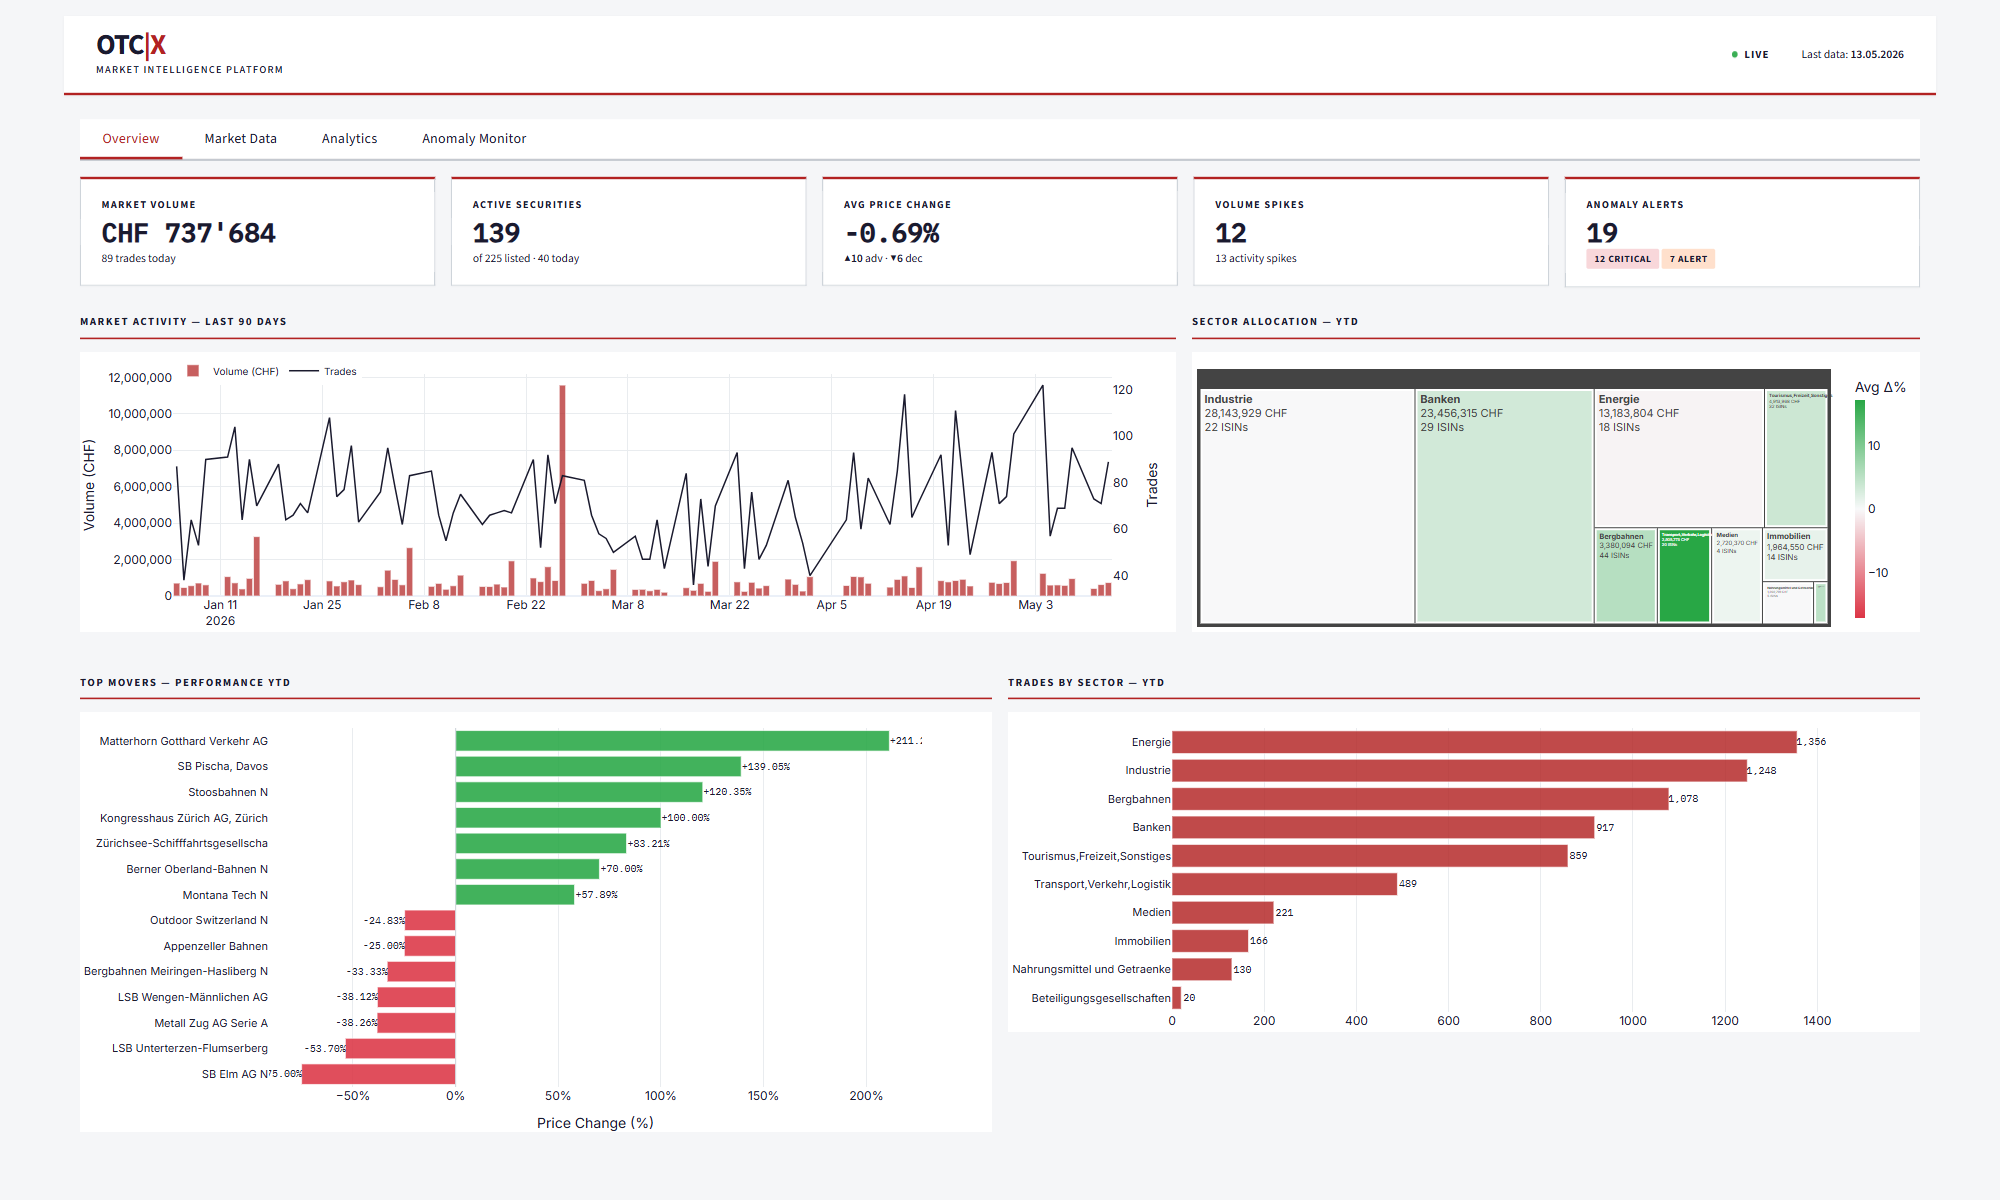
\includegraphics[width=\textwidth]{screenshots/tab1-overview.png}
\caption{Tab 1: Overview\;---\;KPI-Karten, Marktaktivität, Sektor-Treemap}
\label{fig:tab-overview}
\end{figure}

\begin{figure}[H]
\centering
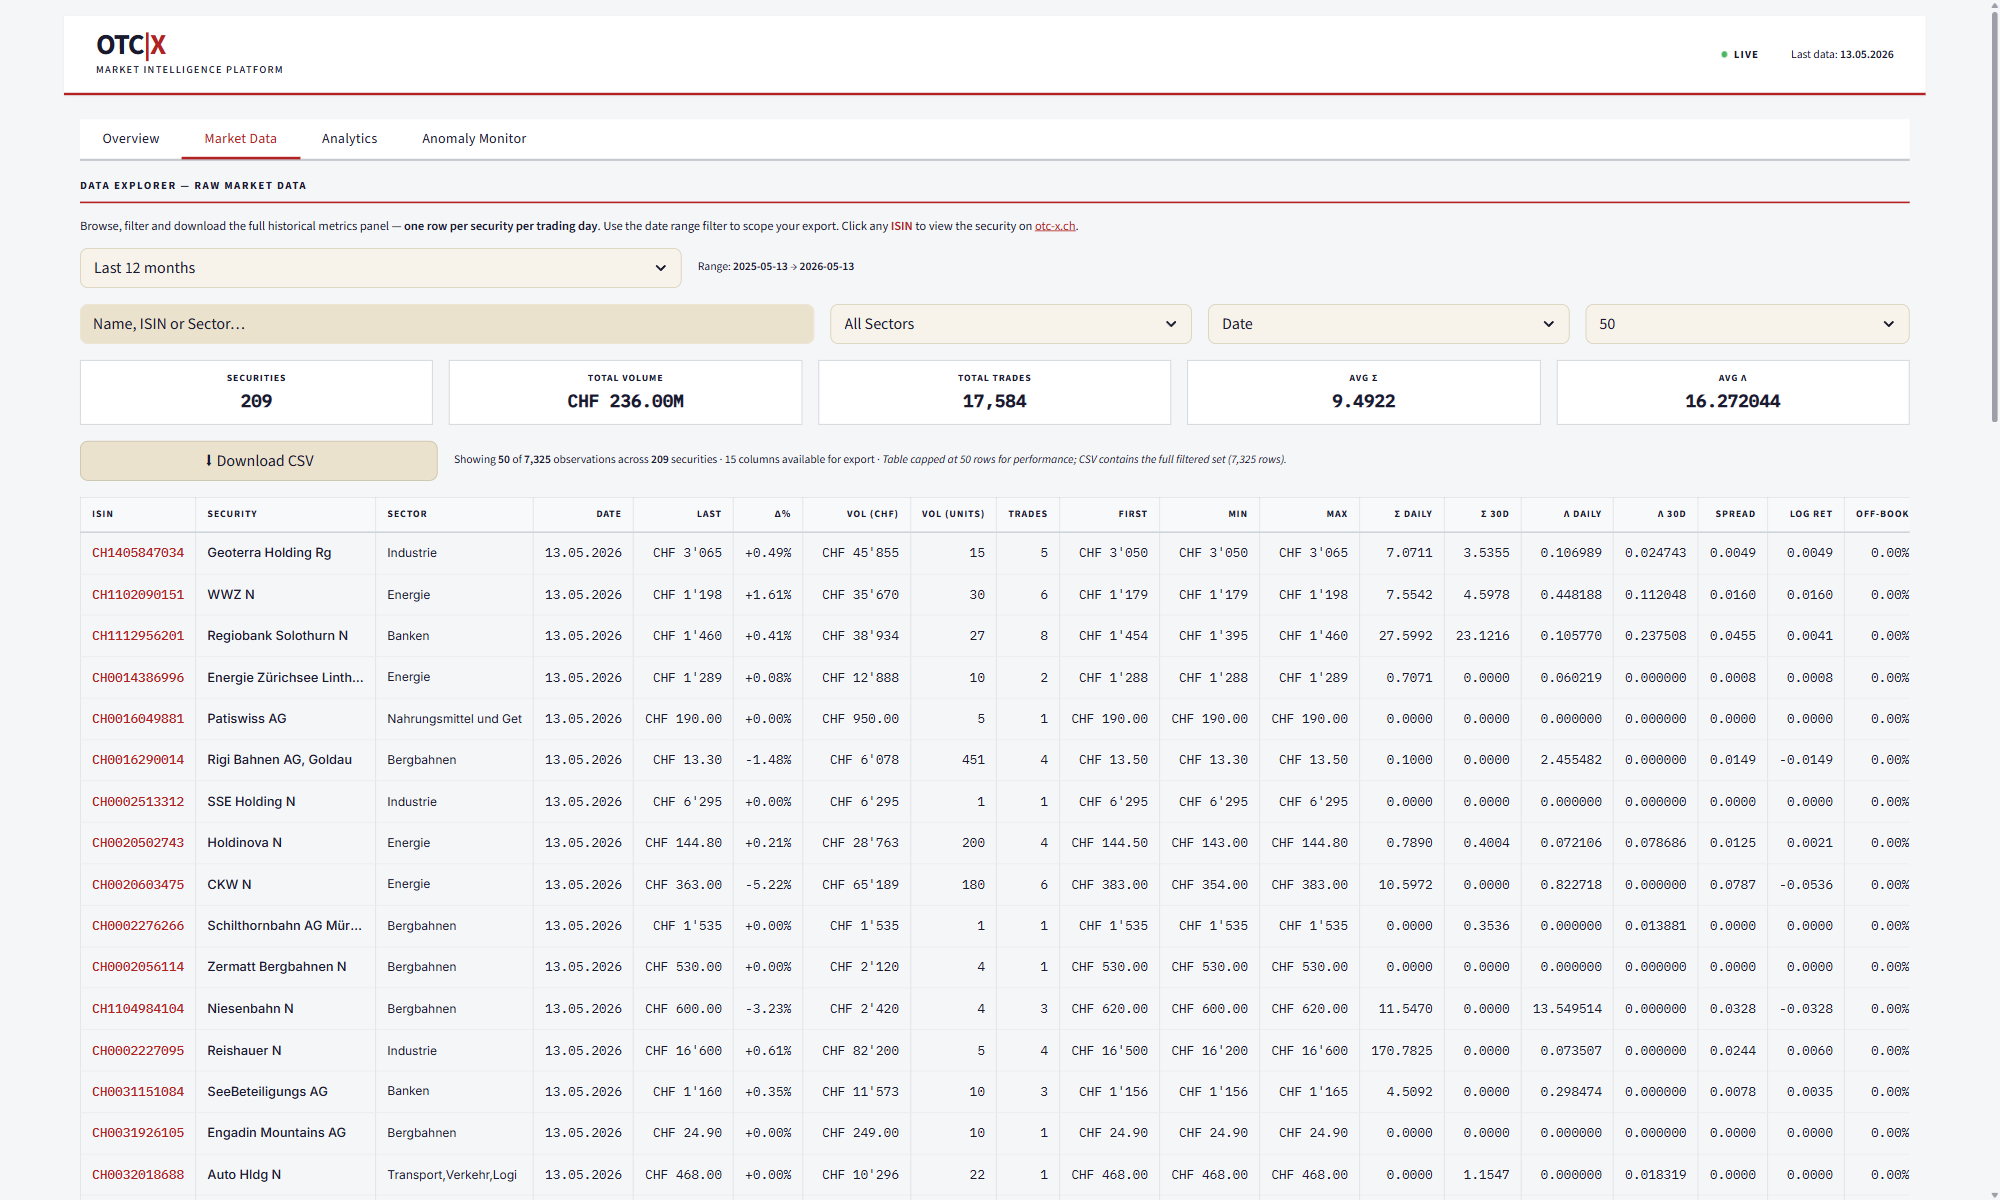
\includegraphics[width=\textwidth]{screenshots/tab2-market-data.png}
\caption{Tab 2: Market Data\;---\;26-Spalten-Explorer mit Suche und Export}
\label{fig:tab-market}
\end{figure}

\begin{figure}[H]
\centering
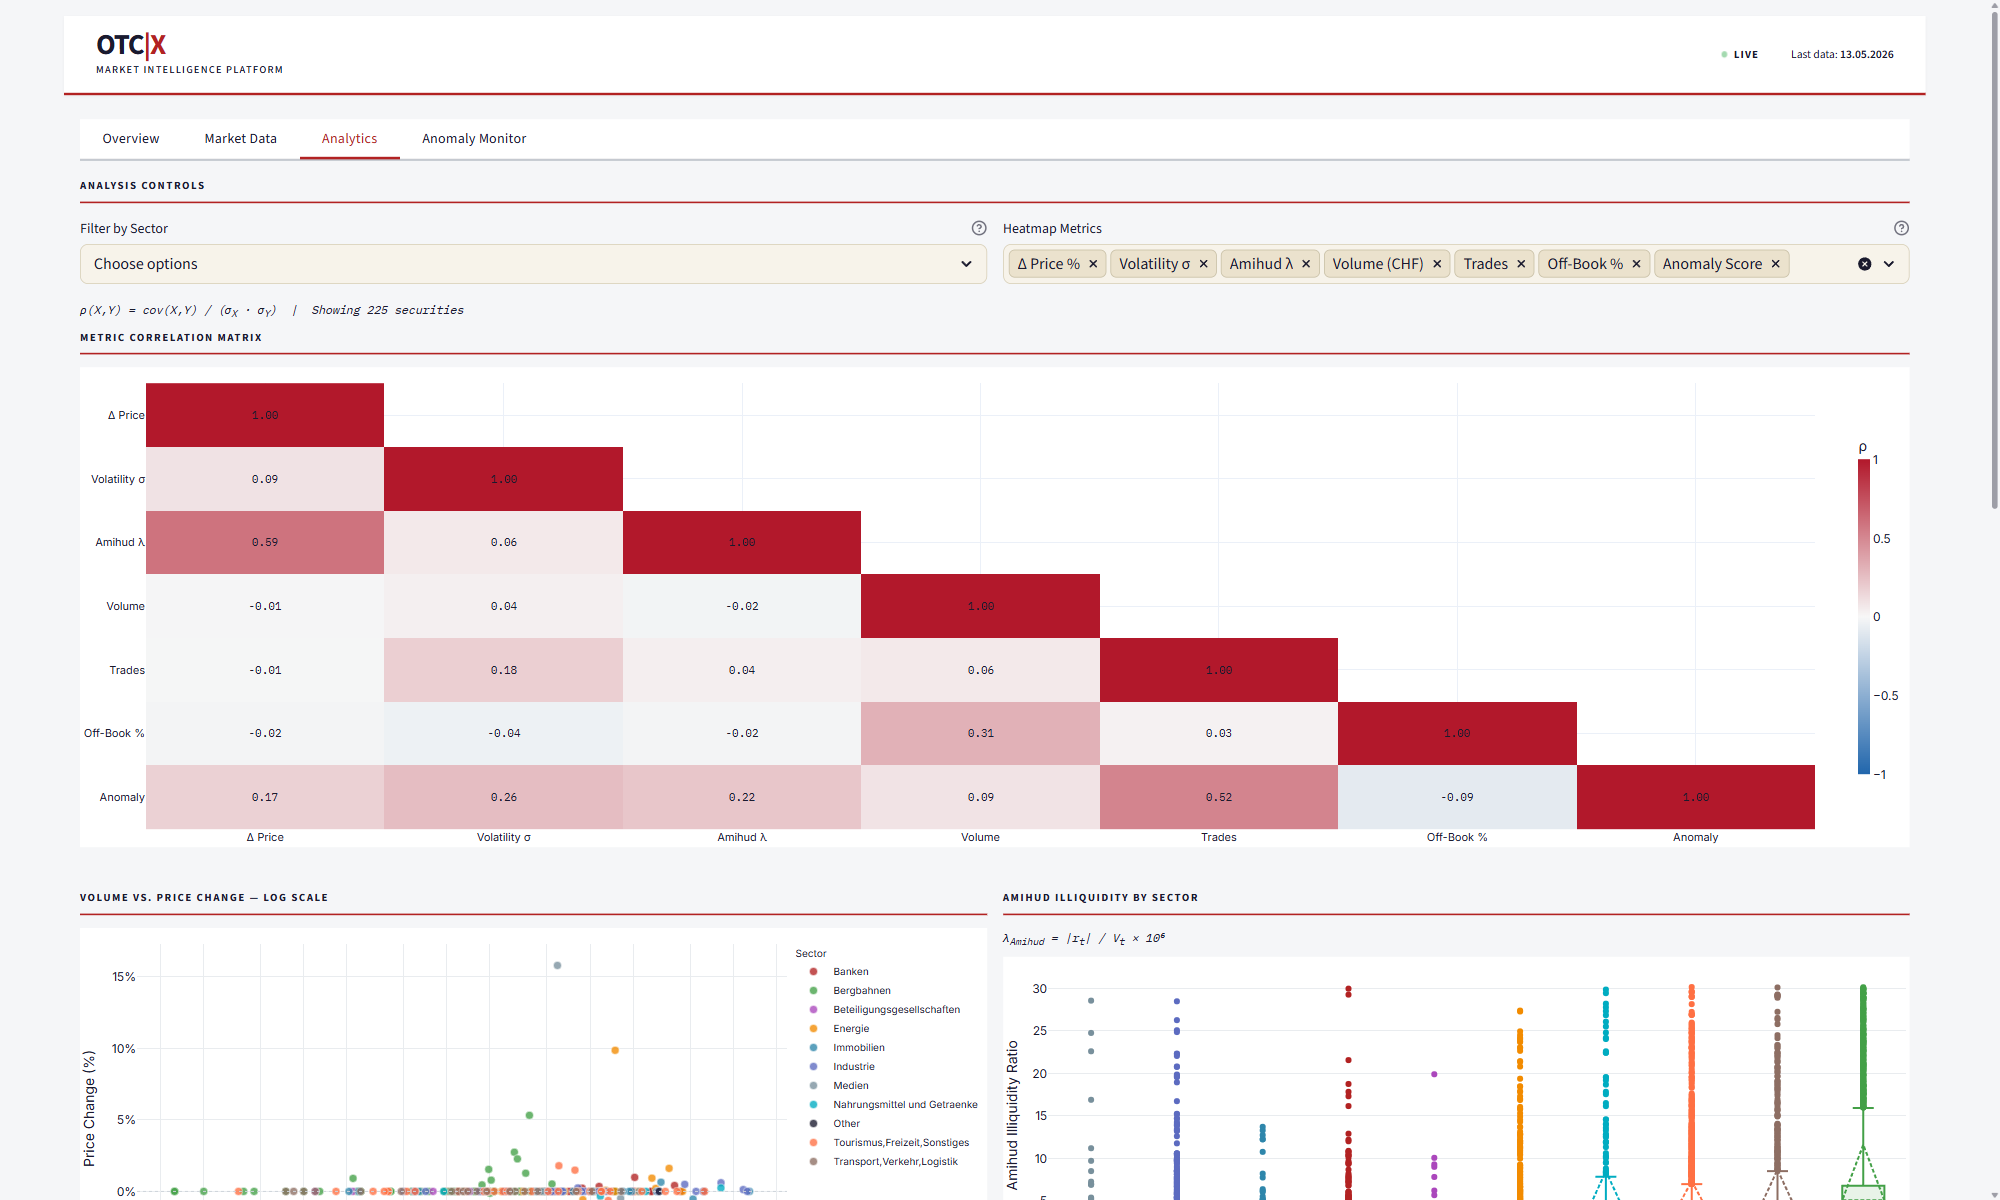
\includegraphics[width=\textwidth]{screenshots/tab3-analytics.png}
\caption{Tab 3: Analytics\;---\;Korrelations-Heatmap, Amihud-Boxplots, 3D-Explorer}
\label{fig:tab-analytics}
\end{figure}

\begin{figure}[H]
\centering
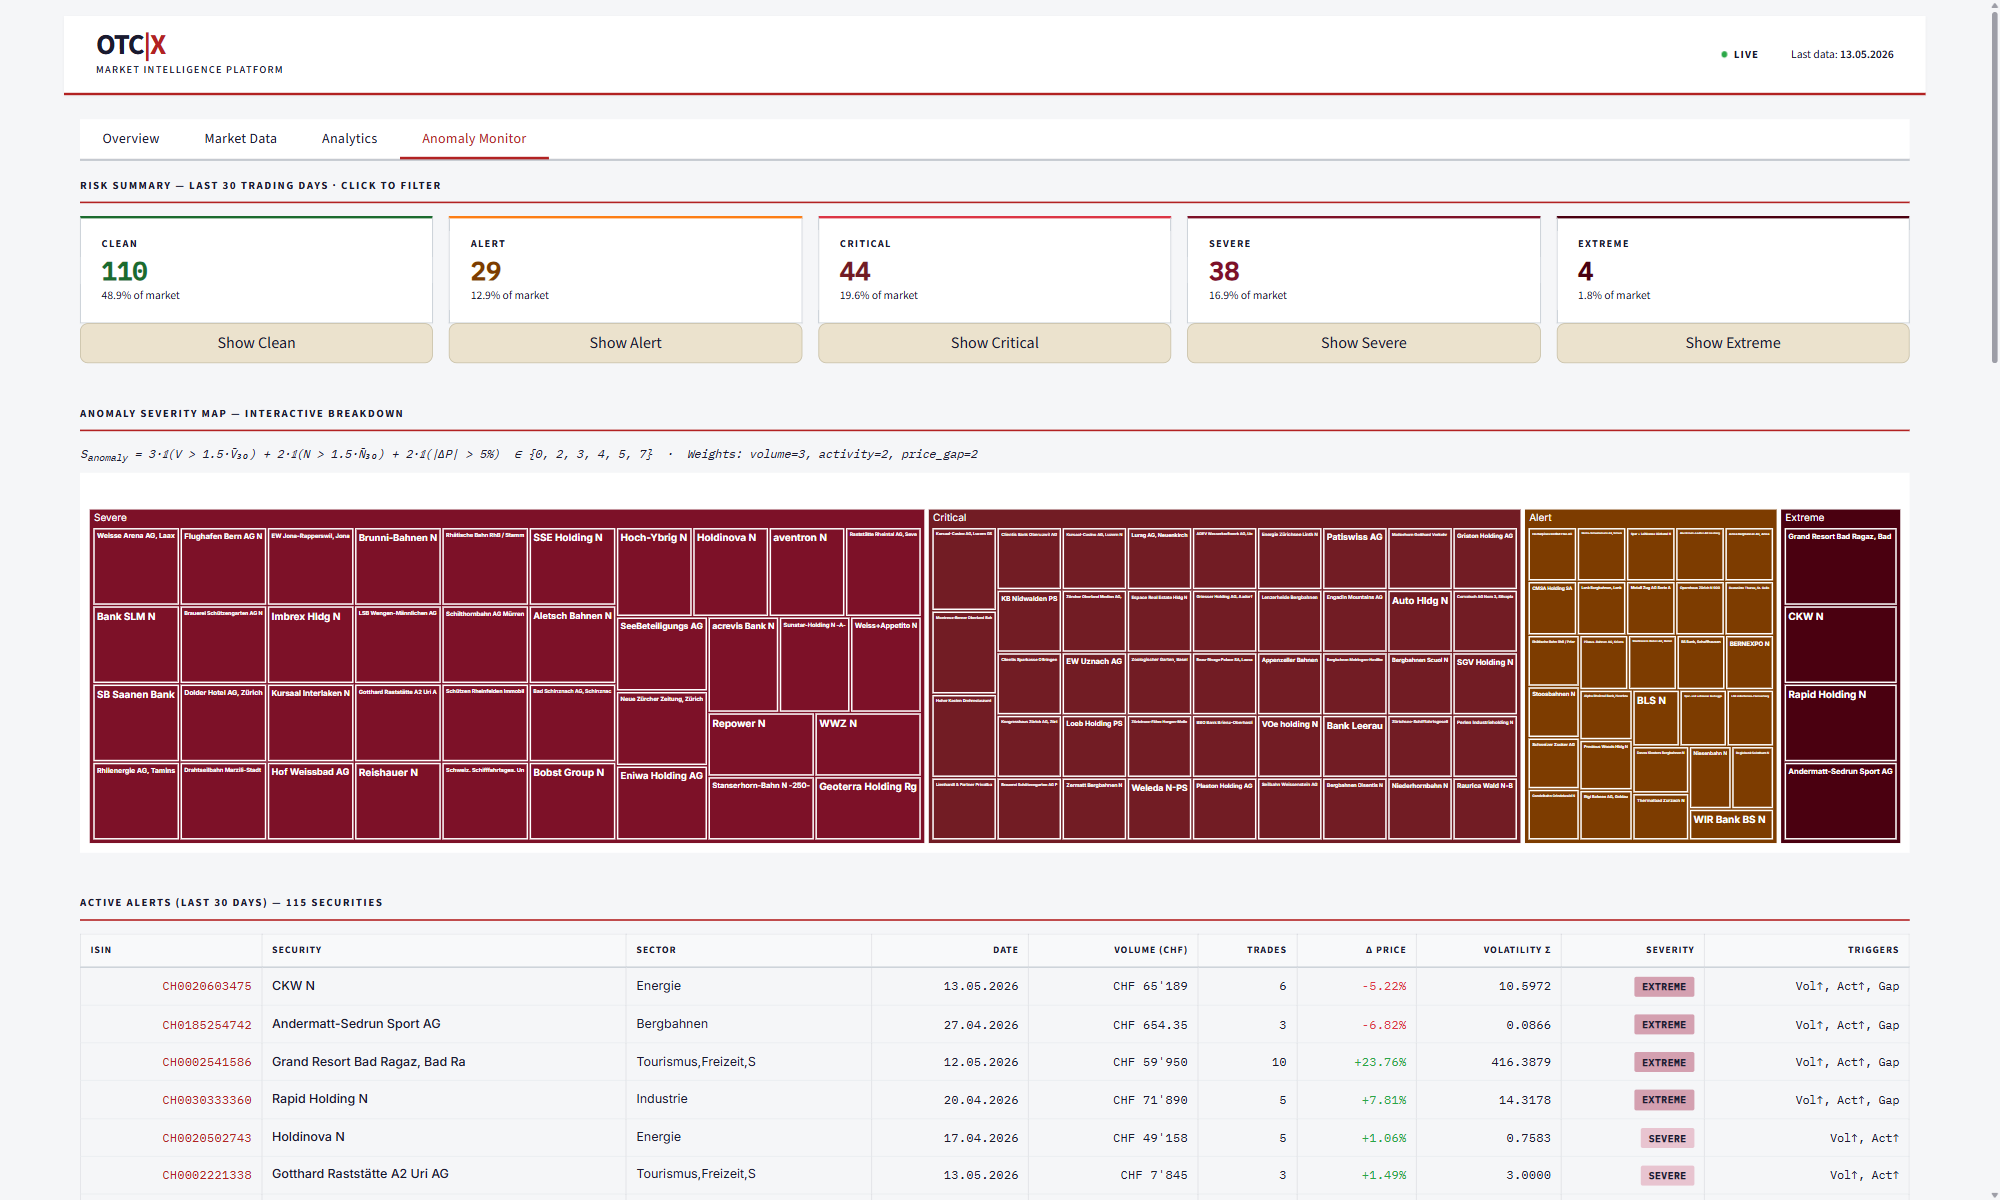
\includegraphics[width=\textwidth]{screenshots/tab4-anomaly-monitor.png}
\caption{Tab 4: Anomaly Monitor\;---\;Severity-Karten und Alert-Tabelle}
\label{fig:tab-anomaly}
\end{figure}


% ═════════════════════════════════════════════════════════════════════════════
%  KAPITEL 7 — QUALITÄTSSICHERUNG
% ═════════════════════════════════════════════════════════════════════════════
\chapter{Qualitätssicherung und Engineering-Standards}
\label{ch:qualitaet}

\epigraph{\itshape Vertrauen entsteht nicht durch Versprechen, sondern durch Verifikation.}{}

\section{Teststrategie}

Die Codebasis wird durch \textbf{115 automatisierte Tests} in fünf Kategorien abgesichert:

\begin{table}[H]
\centering
\caption{Teststruktur nach Modul und Kategorie}
\label{tab:tests}
\rowcolors{2}{LightSilver}{white}
\sffamily\small
\begin{tabularx}{\textwidth}{>{\ttfamily\bfseries}p{3.5cm} l X}
  \toprule
  \rowcolor{DeepNavy} \textcolor{white}{\textbf{Testmodul}} & \textcolor{white}{\textbf{Kategorie}} & \textcolor{white}{\textbf{Abdeckung}} \\
  \midrule
  test\_backend.py     & Unit + Integration   & ISIN-Berechnung (Luhn), Metriken-Engine, Pipeline-Imports \\
  test\_frontend.py    & Unit + Smoke         & Formatierungs-Utilities (CHF, \%, Badge), Config, Chart-Instantiierung \\
  test\_paths.py       & Integration          & Pfadauflösung, Datei-Existenzprüfung über alle Module \\
  test\_integration.py & Integration          & Metriken-Verkettung, Data-Loader-Integration \\
  test\_acceptance.py  & BDD-Akzeptanz        & Geschäftslogik-Validierung via pytest-bdd \\
  \bottomrule
\end{tabularx}
\end{table}

\begin{insightbox}
\textbf{Werttreiber.}\;115 CI-gegatete Tests sind nicht nur Versicherung gegen Regressionen\,---\,sie kodifizieren die \emph{Intention} hinter jeder Berechnung als ausführbaren Vertrag und ermöglichen sichere Erweiterung durch Folgeentwickler. Der Daily-Pipeline-Workflow führt die Testsuite \emph{vor} dem Daten-Refresh aus; ein fehlgeschlagener Test verhindert die Veröffentlichung potenziell fehlerhafter Marktdaten.
\end{insightbox}

\section{Code-Konventionen}

\begin{itemize}
  \item \textbf{Type Hints:}\;Sämtliche Funktionssignaturen tragen vollständige Typannotationen (PEP\,484).
  \item \textbf{Docstrings:}\;NumPy-Style mit \code{Parameters}, \code{Returns}, \code{Raises} und \code{Notes}-Sektionen.
  \item \textbf{Pfadauflösung:}\;Ausschliesslich via \code{Path(\_\_file\_\_).resolve().parent}-Ketten; keine hardcodierten Pfade.
  \item \textbf{Zahlenformatierung:}\;Schweizer Konventionen (Apostroph als Tausendertrenner, CHF-Währung).
  \item \textbf{Backend/Frontend-Separation:}\;Backend nutzt Polars; Frontend nutzt Pandas. Keine Vermischung.
\end{itemize}

\section{Pfadauflösungsstrategie}

\begin{lstlisting}[language=Python, caption={Pfadauflösungsmuster\;---\;keine hartcodierten Pfade}]
from pathlib import Path

# Backend: ein Parent hoch von operations/ zu backend/
script_dir = Path(__file__).resolve().parent
data_dir   = script_dir.parent / "data"

# Frontend: drei Parents hoch zur Wurzel, dann in backend/data/
root     = Path(__file__).resolve().parent.parent.parent
data_dir = root / "backend" / "data"
\end{lstlisting}


% ═════════════════════════════════════════════════════════════════════════════
%  KAPITEL 8 — STRATEGISCHER FAHRPLAN UND ROADMAP
% ═════════════════════════════════════════════════════════════════════════════
\chapter{Strategischer Fahrplan und Roadmap}
\label{ch:roadmap}

\epigraph{\itshape Eine Roadmap ist kein Versprechen\,---\,sondern die Disziplin, mit der eine Vision in Quartale zerlegbar wird.}{}

Die in Abschnitt~\ref{sec:roadmap-teaser} skizzierten strategischen Säulen werden hier in eine konkrete Sequenz mit Quartal-Granularität, Abhängigkeiten und Erfolgskriterien überführt. Der Fahrplan dient als Diskussionsgrundlage gegenüber den Stakeholdern; Termine sind Indikationen für die Planung, nicht vertragliche Zusagen.

% ── Roadmap Gantt — single visual replacing 4 stacked phase tables ─────────
\begin{figure}[H]
\centering
\sffamily\footnotesize
\begin{ganttchart}[
  hgrid={draw=N300, line width=0.3pt},
  vgrid={*{2}{draw=N300, dotted}, *{1}{draw=N400, line width=0.4pt}},
  x unit=4mm,
  y unit chart=6mm,
  y unit title=6mm,
  title height=1,
  bar height=0.65,
  bar top shift=0.18,
  bar/.style={fill=MetricBlue, draw=DeepNavy, line width=0.3pt},
  bar label font=\sffamily\footnotesize,
  bar label node/.style={text width=42mm, align=right, font=\sffamily\footnotesize\color{N800}},
  group/.style={fill=DeepNavy, draw=DeepNavy},
  group label font=\sffamily\bfseries\footnotesize\color{DeepNavy},
  milestone/.style={fill=SwissRed, draw=SwissRed},
  milestone label font=\sffamily\footnotesize\color{SwissRed},
  title/.style={fill=N100, draw=N400, line width=0.3pt},
  title label font=\sffamily\bfseries\small\color{DeepNavy},
  inline,
]{1}{28}
  % Time axis: 2026 Q2-Q4 + 2027 Q1-Q4 + 2028+
  \gantttitle{2026}{9} \gantttitle{2027}{12} \gantttitle{2028\,+}{7} \\
  \gantttitle{Q2}{3} \gantttitle{Q3}{3} \gantttitle{Q4}{3}
  \gantttitle{Q1}{3} \gantttitle{Q2}{3} \gantttitle{Q3}{3} \gantttitle{Q4}{3}
  \gantttitle{H1}{3} \gantttitle{H2+}{4} \\
  % Phases
  \ganttbar{Phase 0 — Foundation \textcolor{SevClean}{✓}}{1}{3} \\
  \ganttbar{Phase 1 — Prädiktive Analytik}{4}{9}
  \ganttmilestone[milestone label node/.append style={anchor=west, xshift=2mm}]{}{9} \\
  \ganttbar{Phase 2 — Marktübergr.\ Anreicherung}{10}{15}
  \ganttmilestone{}{15} \\
  \ganttbar{Phase 3 — Echtzeit-Streaming}{16}{21}
  \ganttmilestone{}{21} \\
  \ganttbar{Phase 4+ — Plattform-Expansion}{22}{28} \\
  % Dependency arrows
  \ganttlink{elem2}{elem3}
  \ganttlink{elem3}{elem4}
  \ganttlink{elem4}{elem5}
\end{ganttchart}
\caption{Strategischer Fahrplan — 5 Phasen mit Meilensteinen und Abhängigkeiten. Phase 0 abgeschlossen, im täglichen Produktivbetrieb. Rote Diamanten markieren Phasen-Abschluss-Meilensteine.}
\label{fig:roadmap-gantt}
\end{figure}

\section{Phase 0\;---\;Foundation (abgeschlossen, im Produktivbetrieb)}

Die heutige Plattform stellt das tragende Fundament dar. Folgende Bausteine sind operativ und werden täglich durch automatisierte CI-Läufe verifiziert:

\begin{itemize}
  \item Vollautomatisierte 4-Stufen-Datenpipeline (täglich 05:00\,UTC seit 29.\,März 2026; aktuell 54 konsekutive Läufe)
  \item 26-spaltige Metriken-Engine mit Amihud-$\lambda$, Corwin--Schultz-Spread-Proxy, dreistufiger EWMA-Volatilitätskaskade
  \item Gewichtetes Anomalie-Scoring mit sechs Severity-Stufen
  \item 4-Tab-Streamlit-Dashboard mit 11 interaktiven Plotly-Charttypen
  \item 115 automatisierte Tests (pytest + pytest-bdd) als CI-Gate
  \item Banking-Grade Container-Distribution (cosign, SBOM, SLSA-Provenance\,---\,siehe~\ref{sec:supplychain})
  \item IREB-konforme Anforderungs-Dokumentation mit Traceability Matrix
\end{itemize}

\section{Phase 1\;---\;Prädiktive Analytik (Q3--Q4 2026)}

\begin{table}[H]
\centering
\caption{Phase 1\,---\,Prädiktive Liquiditätsprognosen}
\label{tab:phase1}
\rowcolors{2}{LightSilver}{white}
\sffamily\small
\begin{tabularx}{\textwidth}{>{\bfseries\sffamily\color{SwissRed}}p{2.4cm} X}
  \toprule
  \rowcolor{DeepNavy} \textcolor{white}{\textbf{Aspekt}} & \textcolor{white}{\textbf{Inhalt}} \\
  \midrule
  Ziel          & Forward-Looking Severity-Score über 24--72\,h Horizont; Prognose-Spalten im täglichen Metrik-Layer \\
  Methodik      & ARIMA für Volumenprognosen, GARCH(1,1) für Volatilitätsprognose, Prophet für saisonale Komponenten; Ensemble-Aggregation mit nightly Backtest-Framework und Rolling-Window-Validierung \\
  Lieferung     & Neue \texttt{forecast\_*}-Spalten im Parquet-Schema; zusätzliches Tab \glqq Forecast\grqq{} im Dashboard mit Konfidenzbändern \\
  Erfolgs\-kriterium & MAE der Volumenprognose $\leq$ 30\,\% des 30-Tage-Medians über Backtest-Universum; reproduzierbare Backtests via CI \\
  Abhängig\-keit & \texttt{statsmodels} und \texttt{prophet} als neue Laufzeitabhängigkeiten\,---\,erfordert formelle Lockerung von Constraint~C-02 durch den Stakeholder \\
  Risiken       & Strukturelle Brüche während illiquider Phasen; Übermodellierung bei dünn gehandelten Titeln; Konfidenzkommunikation gegenüber Endnutzern \\
  \bottomrule
\end{tabularx}
\end{table}

\section{Phase 2\;---\;Marktübergreifende Anreicherung (Q1--Q2 2027)}

\begin{table}[H]
\centering
\caption{Phase 2\,---\,Cross-Market-Kontextualisierung}
\label{tab:phase2}
\rowcolors{2}{LightSilver}{white}
\sffamily\small
\begin{tabularx}{\textwidth}{>{\bfseries\sffamily\color{SwissRed}}p{2.4cm} X}
  \toprule
  \rowcolor{DeepNavy} \textcolor{white}{\textbf{Aspekt}} & \textcolor{white}{\textbf{Inhalt}} \\
  \midrule
  Ziel          & OTC-Bewegungen im Kontext des gesamten Schweizer Finanzökosystems einordnen; Konzentrationsrisiken über Marktsegmente hinweg quantifizieren \\
  Methodik      & Integration von SIX Swiss Exchange Referenzdaten (kotierte Peers), SNB-Leitzinsen, KOF-Konjunkturbarometer, CPI; computational Pairs-Trading-Indikatoren OTC vs.\ kotiert; sektorbasierte Beta-Berechnung \\
  Lieferung     & Neues Tab \glqq Cross-Market Context\grqq{}; angereicherte Korrelations-Heatmap mit kotierten Vergleichstiteln; makroökonomische Hintergrund-Overlays in Zeitreihen \\
  Erfolgs\-kriterium & Mindestens 80\,\% der 243 OTC-Titel mit kotiertem Peer-Mapping versehen; sektorale Beta-Werte mit $R^2 \geq 0{,}3$ \\
  Abhängig\-keit & SIX-Datenzugang (kommerzielle Lizenz oder Datapool-Mitgliedschaft erforderlich); Stabilität der SNB-Daten-API \\
  Risiken       & Lizenz-Kostenkomponente; Asynchronität zwischen OTC- und SIX-Tagesabschlüssen; Datenqualität von Drittquellen \\
  \bottomrule
\end{tabularx}
\end{table}

\section{Phase 3\;---\;Echtzeit-Streaming (Q3--Q4 2027)}

\begin{table}[H]
\centering
\caption{Phase 3\,---\,Sub-Tages-Latenz}
\label{tab:phase3}
\rowcolors{2}{LightSilver}{white}
\sffamily\small
\begin{tabularx}{\textwidth}{>{\bfseries\sffamily\color{SwissRed}}p{2.4cm} X}
  \toprule
  \rowcolor{DeepNavy} \textcolor{white}{\textbf{Aspekt}} & \textcolor{white}{\textbf{Inhalt}} \\
  \midrule
  Ziel          & Signal-Latenz von $\approx 24$\,h auf $< 5$\,Min reduzieren; Intraday-Severity-Updates und ereignisgetriebene Alerts \\
  Methodik      & WebSocket-basierte Tick-Aufnahme (sofern OTC-X-API erweitert), inkrementelle Aggregation im Apache-Arrow-Streaming-Format, persistente Online-Metriken via Polars LazyFrames \\
  Lieferung     & Live-Anomalie-Indikator im Dashboard; optional Push-Notifications (E-Mail/Mobile) bei Schwellüberschreitung; SLA-fähige Tick-zu-Signal-Latenz-Metriken \\
  Erfolgs\-kriterium & End-to-End Tick-zu-Severity-Update-Latenz $< 5$\,Min für 95\,\% aller Events \\
  Abhängig\-keit & Erweiterung der OTC-X-API durch BEKB / Berner Börse (heute ausschliesslich Tagesexporte verfügbar) \\
  Risiken       & Ohne API-Erweiterung nur durch Polling-Approximation erreichbar; betrieblicher Overhead durch 24/7-Verfügbarkeitserwartung; höhere Hostingkosten \\
  \bottomrule
\end{tabularx}
\end{table}

\section{Über die drei Säulen hinaus\;---\;Plattform-Expansion (ab 2028)}

Im Falle einer allfälligen formellen Übernahme durch einen institutionellen Träger öffnet sich der Möglichkeitsraum für eine breitere Plattform-Positionierung. Diese Optionen werden \emph{ohne} Festlegung skizziert\,---\,die Entscheidung obläge dem künftigen Träger:

\begin{itemize}
  \item \textbf{Multi-Mandanten-Fähigkeit}\,---\,nach Lizenz-Klärung Lizenzierung an institutionelle Drittnutzer (Vermögensverwalter, Family Offices, Sektor-Analysten).
  \item \textbf{Plattform-Generalisierung}\,---\,Adaption der Methodik auf weitere illiquide Märkte: Privatmarktinstrumente, alternative Anlageklassen, ausländische OTC-Plätze (z.\,B. Wiener Direkthandel, Frankfurter Freiverkehr).
  \item \textbf{Programmatischer API-Layer}\,---\,REST/GraphQL-Zugriff auf Metriken und Anomalie-Signale für Algorithmic-Trading-Integrationen.
  \item \textbf{Forschungs-Kooperationen}\,---\,Zusammenarbeit mit FHNW, Universität Bern oder ETH zur Veröffentlichung der quantitativen Methodik in peer-reviewed Journals (Anonymisierung der proprietären Daten vorausgesetzt).
\end{itemize}

\begin{insightbox}
Die übergeordnete Ambition besteht darin, OTC-X nicht bloss als retrospektives Analysewerkzeug zu etablieren, sondern als \textbf{vorausschauendes Entscheidungsunterstützungssystem für institutionelle Akteure auf illiquiden Märkten}\,---\,ein Wächter, der den Schweizer OTC-Markt beobachtet, damit Händler es nicht mehr eigenhändig tun müssen, und eine generalisierbare Methodik, die diese Disziplin auf weitere intransparente Marktsegmente überträgt.
\end{insightbox}


% ═════════════════════════════════════════════════════════════════════════════
%  KAPITEL 9 — GLOSSAR UND REFERENZEN
% ═════════════════════════════════════════════════════════════════════════════
\chapter{Glossar und Referenzen}
\label{ch:glossar}

\section{Fachbegriffe}

\begin{table}[H]
\centering
\rowcolors{2}{LightSilver}{white}
\sffamily\small
\begin{tabularx}{\textwidth}{>{\bfseries\sffamily}p{3.5cm} X}
  \toprule
  \rowcolor{DeepNavy} \textcolor{white}{\textbf{Begriff}} & \textcolor{white}{\textbf{Definition}} \\
  \midrule
  Amihud-Ratio ($\lambda$) & Mass für den Preisimpakt pro gehandelte Volumeneinheit; hohe Werte indizieren Illiquidität \\
  Anomaly Score             & Gewichteter Composite-Wert ($S \in \{0,2,3,4,5,7\}$) aus drei binären Flags \\
  Corwin--Schultz Proxy     & Approximation der Geld-Brief-Spanne via logarithmisches Hoch-Tief-Verhältnis \\
  EWMA                      & Exponentially Weighted Moving Average; gewichtete Glättung mit Vergangenheitsdämpfung \\
  IREB                      & International Requirements Engineering Board; Zertifizierungsstandard für RE \\
  ISIN                      & International Securities Identification Number; 12-stelliger alphanumerischer Code \\
  Luhn-Algorithmus          & Prüfzifferverfahren nach ISO~7812 zur Validierung von Identifikationsnummern \\
  OTC-X                     & Ausserbörsliche Handelsplattform der Berner Kantonalbank für Schweizer Titel \\
  Parquet                   & Spaltenorientiertes Speicherformat für analytische Workloads (Apache Foundation) \\
  Polars                    & Hochperformante DataFrame-Engine in Rust mit Python-Bindings \\
  Rolling Median            & Gleitender Median über ein definiertes Zeitfenster; robust gegenüber Ausreissern \\
  Severity-Tier             & Klassifikationsstufe (Clean bis Extreme) basierend auf dem Composite Anomaly Score \\
  Valor                     & Schweizerische Wertpapieridentifikationsnummer (6--7 Ziffern) \\
  \bottomrule
\end{tabularx}
\end{table}

\section{Literatur und Standards}

\begin{enumerate}
  \item Amihud, Y. (2002). \textit{Illiquidity and stock returns: cross-section and time-series effects.} Journal of Financial Markets, 5(1), 31--56.
  \item Corwin, S.\,A. \& Schultz, P. (2012). \textit{A simple way to estimate bid-ask spreads from daily high and low prices.} The Journal of Finance, 67(2), 719--760.
  \item IREB (2023). \textit{Certified Professional for Requirements Engineering -- Foundation Level Syllabus}, Version~3.1.2. International Requirements Engineering Board.
  \item ISO~6166:2021. \textit{Financial services -- International securities identification number (ISIN)}.
  \item ISO~7812-1:2017. \textit{Identification cards -- Identification of issuers -- Part 1: Numbering system} (Luhn).
  \item ISO~9241-210:2019. \textit{Ergonomics of human-system interaction -- Part 210: Human-centred design}.
  \item McKinney, W. (2017). \textit{Python for Data Analysis}, 2nd ed. O'Reilly Media.
  \item Ritchie, J. et al. (2024). \textit{Polars: Blazingly fast DataFrames in Rust and Python.} \url{https://pola.rs}
\end{enumerate}


% ═════════════════════════════════════════════════════════════════════════════
%  ANHANG
% ═════════════════════════════════════════════════════════════════════════════
\appendix

\chapter{Output-Schema-Referenz}
\label{app:schema}

\begin{longtable}{c >{\ttfamily}l l p{6cm}}
\caption{Vollständiges Schema von \code{daily\_metrics.parquet} (26~Spalten)} \\
\toprule
\textbf{\#} & \textbf{Spalte} & \textbf{Typ} & \textbf{Beschreibung} \\
\midrule
\endfirsthead
\caption[]{(Fortsetzung)} \\
\toprule
\textbf{\#} & \textbf{Spalte} & \textbf{Typ} & \textbf{Beschreibung} \\
\midrule
\endhead
\bottomrule
\endfoot
\rowcolor{LightSilver}
1  & Isin                  & String   & International Securities Identification Number \\
2  & Name                  & String   & Unternehmensname (aus Wertpapier-Metadaten) \\
\rowcolor{LightSilver}
3  & Sektor                & String   & Wirtschaftliche Sektorklassifikation \\
4  & Datum                 & Date     & Handelstag \\
\rowcolor{LightSilver}
5  & trades\_today          & UInt32   & Anzahl Trades an diesem Tag \\
6  & volume\_today\_units    & Float64  & Gesamtvolumen in Stück \\
\rowcolor{LightSilver}
7  & volume\_today\_chf      & Float64  & Gesamtvolumen in CHF \\
8  & price\_min             & Float64  & Intraday-Tiefstkurs \\
\rowcolor{LightSilver}
9  & price\_max             & Float64  & Intraday-Höchstkurs \\
10 & price\_first           & Float64  & Eröffnungskurs (erster Trade) \\
\rowcolor{LightSilver}
11 & price\_last            & Float64  & Schlusskurs (letzter Trade) \\
12 & price\_change\_pct      & Float64  & Tägliche Preisveränderung (\%) \\
\rowcolor{LightSilver}
13 & log\_returns           & Float64  & Natürlicher Logarithmus des Kursverhältnisses \\
14 & volatility\_daily      & Float64  & Intraday-Standardabweichung der Kurse \\
\rowcolor{LightSilver}
15 & amihud\_daily          & Float64  & Amihud-Illiquiditätsratio ($\lambda$) \\
16 & spread\_log\_hl         & Float64  & Logarithmischer High-Low Spread Proxy \\
\rowcolor{LightSilver}
17 & trade\_duration\_min    & Float64  & Maximale Lücke zwischen konsekutiven Trades (Min.) \\
18 & off\_book\_pct          & Float64  & Anteil Off-Book-Trades (\%) \\
\rowcolor{LightSilver}
19 & trades\_30d\_median     & Float64  & 30-Handelstage-Rolling-Median der Trade-Anzahl \\
20 & volume\_30d\_median     & Float64  & 30-Handelstage-Rolling-Median des CHF-Volumens \\
\rowcolor{LightSilver}
21 & volatility\_30d\_median & Float64  & 30-Handelstage-Rolling-Median der Volatilität \\
22 & amihud\_30d\_median     & Float64  & 30-Handelstage-Rolling-Median des Amihud $\lambda$ \\
\rowcolor{LightSilver}
23 & volume\_spike          & Boolean  & Flag: $V > 1{,}5 \times \tilde{V}_{30}$ \\
24 & activity\_spike        & Boolean  & Flag: $N > 1{,}5 \times \tilde{N}_{30}$ \\
\rowcolor{LightSilver}
25 & price\_gap             & Boolean  & Flag: $|\Delta P\%| > 5$ \\
26 & anomaly\_score         & UInt8    & Composite Anomaly Score $\in [0, 7]$ \\
\end{longtable}


\chapter{Abkürzungsverzeichnis}
\label{app:abkuerzungen}

\printglossary[type=\acronymtype, title={}, nonumberlist]


% ═════════════════════════════════════════════════════════════════════════════
%  KOLOPHON
% ═════════════════════════════════════════════════════════════════════════════
\vfill

\begin{center}
{\color{SwissRed}\rule{0.5\textwidth}{1pt}}

\vspace{0.6cm}
{\sffamily\textcolor{DeepNavy}{\textbf{OTC\,|\,X}}\;\textcolor{SlateGrey}{·\;Liquidity Intelligence Radar\;·\;Swiss OTC Market}}

\vspace{0.3cm}
{\small\sffamily\textcolor{SlateGrey}{Dieses Dokument ist Bestandteil des proprietären OTC-X Projekts.}}\\[3pt]
{\small\sffamily\textcolor{SlateGrey}{\copyright{} 2026 Mihael Atanasov\;·\;\href{mailto:mihaelatanasov22@gmail.com}{mihaelatanasov22@gmail.com}\;·\;Alle Rechte vorbehalten.}}\\[3pt]
{\small\sffamily\textcolor{SlateGrey}{Unabhängig erstellt; der Berner Kantonalbank AG unverbindlich zur Kenntnisnahme überreicht.}}

\vspace{0.3cm}
{\footnotesize\sffamily\textcolor{SlateGrey}{Mit Präzision gefertigt\;\;$\bullet$\;\;für den Schweizer OTC-Markt}}

\vspace{0.5cm}
{\color{SwissRed}\rule{0.5\textwidth}{1pt}}
\end{center}

\end{document}
